%: ----------------------- introduction file header -----------------------
% the code below specifies where the figures are stored
\graphicspath{{5/figures/}}

\chapter{Automatic Chord Estimation}
\label{chp:chord_estimation}

% Context / Purpose
The previous chapter was able to reformulate timbre similarity as a well-defined task that used objective information for development and evaluation.
Automatic chord recognition, one of the oldest subtopics in the field of content-based MIR, embodies nearly the polar opposite scenario, being rather ill-defined and depending on subjective information almost exclusively.
As such, it provides an interesting case study with which to test the limits of deep learning.
% Goal
In addition to the standard objective of looking to advance the state of the art in a chosen application domain, this chapter seeks to explore the limitations of deep learning as applied to complex music intelligence task.
A thorough investigation serves to not only offer insight into the application of deep learning methods to future problems in content-based MIR, but also culminate in a better understanding of the chord estimation task itself.


\section{Context}
\label{sec:context}

In this section, the prerequisite knowledge necessary to appreciate a thorough treatment of automatic chord estimation systems is addressed.
% Concepts - Build an understanding of musical harmony
First, a basic review of Western tonal theory sets out to define key music concepts, and thus provides a language with which to discuss the problem.
% Practical considerations - Chord syntax
This is followed by a brief outline of the syntax used here to compactly notate chords.
% Motivation -- why
The problem domain is then jointly motivated by potential use-cases and the observed needs of online music communities.
% Limitations -- caveats
Finally, known limitations are detailed to contextualize both assumptions and any conclusions drawn from this work.



\subsection{Musical Foundations}
\label{subsec:musical_foundations}

% Acoustics and perceptions -- pitch, tones, octaves, frequency
% -------------------------
To understand the chord estimation task is to understand the concepts on which it is built.
% To get to the top, start at the bottom.
The most atomic unit in the acoustic realm of chords is a \emph{tone}, defined here as a pitched sound object.
Pitch is defined as the perceptual phenomena whereby a sound stimulus can be matched to the frequency of a pure sinusoid, known as the fundamental frequency.
As a result, sounds can be naturally ordered by fundamental frequency on a scale from low to high.
An \emph{octave} is defined as the doubling of a quantity, and exhibits a special relationship in human perception by which two tones, differeing in fundamental frequency by an integer power of 2, are perceived as being similar; this phenomena is referred to as octave equivalence \cite{?}.
% Pitch helix here?

% Notes and tuning systems
% ------------------------
A \emph{note} is the musical counterpart of a tone, and the two are related by way of a tuning system.
While there are a multiplicity of tuning systems, this work will exclusively consider 12-Tone Equal Temperament, or 12-TET, named for the 12 discrete, equally spaced tones between within an octave.
The relationship between notes and tones in 12-TET is defined by the following:

\begin{equation}
\label{eq:tuning}
f_{pitch} = f_{tuning} * 2 \exp(\frac{n_{index} - 48}{N})
\end{equation}

\noindent where $N$ is the number of notes per octave, $n_{index}$ is an integer note index, $f_{tuning}$ is the reference frequency, in Hertz, on which , and $f_{pitch}$ is the fundamental frequency, in Hertz, of the corresponding tone.
In 12-TET, the \emph{unique pitch classes} within an octave are named, given by the ordered set, $\mathcal{P}$:

\begin{equation}
\label{eq:pitch_classes}
\mathcal{P} = \{C, C\sharp / D\flat, D, D\sharp / E\flat, E, F, F\sharp / G\flat, G, G\sharp / A\flat, A, A\sharp / B\flat, B\}
\end{equation}

Here, sharps, $\sharp$, and flats, $\flat$, are symbols used to indicate the raising or lowering of a note by one semitone, respectively.
Note that due to this particular tuning system, some pitch classes can be spelled with either a sharp or a flat, e.g. $A\sharp = B\flat$, a property known as \emph{enharmonic equivalence}.
An absolute note name, consisting of a pitch class, $p$, and an octave, $o$, is given by the following as a function of absolute note index, such that $n_{index}=0~\to~C0$, $n_{index}=12~\to~C1$, etc.:

\begin{align*}
p = \mathcal{P}[mod(n_{index}, 12)] \\
o = \lfloor~n_{index} / 12~\rfloor
\end{align*}

In contemporary music, standard concert tuning equates $A4=440Hz$; classically, the tuning frequency is defined such that it falls in the performance range of a majority of instruments to be matched exactly, and hence the offset in Eq. \ref{eq:tuning}.
% dunno I like / want this sentence
Were the tuning system and reference frequency universally constant, the concepts of tones and notes would be equivalent; it should be noted, however, this is not the case.

% Intervals
% ---------
Most\footnote{But not all, as in the case of John Cage's \emph{4'33''}, which contains none.} real music combines many different notes, and thus it is useful to define an \emph{interval} is defined as the relative semitone distance between two notes.
Whereas notes are atomic, intervals are the bonds in a harmonic molecule.
The interval between consecutive pitch classes is referred to as a \emph{semitone}, with a step size of 1, and a step size of 2 is known as a \emph{whole tone}.
Intervals are critical to music perception because they are generally perceived as similar regardless of pitch height, e.g. the interval from C4 to G4 sounds the same as the interval from F4 to C5, both being seven semitones.

% Scales, chords, and keys; a circular quagmire
% ------------------------
From here, three interdependent harmonic concepts are built through the simultaneous and sequential combination of notes and, as a result, intervals: scales, chords, and keys.
It is crucial to recognize that each is an emergent quality of the same fundamental parts, and efforts to define one in terms of another results in circular logic.
For clarity, the relationships between the various entities discussed so far are diagrammed hierarchically in Figure \ref{fig:concept_hierarchy}.

That said, an ordered set of intervals in known as a scale, of which the \emph{diatonic} is the most widely used in common practice music.
It consists of eight semitone scale degrees, and thus seven intervals, given by the following:

\begin{align*}
\{2, 2, 1, 2, 2, 2, 1\}
\end{align*}

Rotating this sequence circularly results in different \emph{modes}, of which two are common in contemporary popular music: \emph{major}, with a rotation of 0; and \emph{minor}, with a rotation to the right of 3.
Starting from 0, the semitone values of these scales are expressed by the following:

\begin{align*}
\texttt{maj} = \{0, 2, 4, 5, 7, 9, 11, 12\} \\
\texttt{min} = \{0, 2, 3, 5, 7, 8, 10, 12\} \\
\end{align*}

These sequences can be used to recover a scale by circularly indexing the set of pitch classes given in \ref{eq:pitch_classes}.
The starting pitch classon which the scale is based is referred to the \emph{tonic}, and lends its name to the scale.
To illustrate, a C Major and A minor scale are given as follows:

\begin{align*}
\mathcal{C}_{major} = \{C, D, E, F, G, A, B\} \\
\mathcal{A}_{minor} = \{A, B, C, D, E, F, G\} \\
\end{align*}

One should observe that these two scales, with different modes and tonics, are composed of identical notes.
These scales are known as each other's relative major and minor, respectively, and share a strong perceptual affinity.


% \begin{table}[h]
% \begin{center}
% \caption{Degrees, names, semitones, and intervals of the Major (Ionian) scale.}
% \label{tab:diatonic}
% \begin{tabular}{c | c | c | c }
% Degree & Name & Semitones & Interval \\
% \hline
% 1st & Tonic & 0 & -- \\
% 2nd & Supertonic & 2 & +2 \\
% 3rd & Mediant & 4 & +2 \\
% 4th & Subdominant & 5 & +1 \\
% 5th & Dominant & 7 & +2 \\
% 6th & Submediant & 9 & +2 \\
% 7th & Leading Tone & 11 & +2\\
% 8th & Tonic (Octave) & 12 & +1 \\
% \hline
% \end{tabular}
% \end{center}

% Chords, by the book
% -------------------
Proceeding from scales, a \emph{chord} is classically conceived as a simultaneous grouping of notes.
One of the most important chord types in Western tonal theory is the \emph{triad}, on which many other theoretical constructs are built.
Comprised of three notes, a triad is built by taking the second and fourth scale degrees from a chosen starting point, referred to as the root.
For example, this expansion is given for the C-major scale in Table \ref{tab:major_triads}.

\begin{table}[h!]
\begin{center}
\caption{Roman numeral, quality, semitones, and intervals of triads in the Major scale.}
\label{tab:major_triads}
\begin{tabular}{c | c | c | c }
Roman Numeral & Quality & Semitones & Intervals \\
\hline
I & Major & \{0, 4, 7\} & \{+4, +3\}\\
ii & minor & \{2, 5, 9\} & \{+3, +4\}\\
iii & minor & \{4, 7, 7\} & \{+3, +4\}\\
IV & Major & \{5, 9, 12\} & \{+4, +3\}\\
V & Major & \{7, 11, 2\} & \{+4, +3\}\\
vi & minor & \{9, 0, 4\} & \{+3, +4\}\\
vii$^\circ$ & diminished & \{11, 2, 5\} & \{+3, +3\}\\
I & Major & \{0, 4, 7\} & \{+4, +3\}\\
\hline
\end{tabular}
\end{center}
\end{table}

For a given chord, the \emph{root} is defined as the home note on which the intervals are stacked, and the \emph{quality} determined by the relationship of the intervals to the root.
An interval of 4 semitones is known as a \emph{major third} and 3 semitones a \emph{minor third}, sharing a commonality with the third scale degree of the major and minor scales, respectively.
Therefore, the qualities of the first six chords in the table are named for their relationship with the corresponding major and minor scales; the vii$^\circ$ chord, however, is named differently because it contains two minor thirds.

% Key
% ---
Sharing much common ground with scales and chords, a \emph{key} identifies a point of harmonic stability in reference to a tonic and its corresponding triad.
Accordingly, the keys conventionally take one of the pitch classes and either a major or minor quality, e.g. $E-major$ or $C\sharp-minor$.
Key is integral to the discussion here, because its impression or expectation establishes a harmonic framework with which to parse musical information, leading to the understanding of notes and intervals as they relate to scales and chords.


% Attempts to define a chord
While much of this theory can be detailed specifically, real music is by no means so well behaved.
As a result, the practical definition of a ``chord'' is open to some interpretation, and may take multiple meanings.
For example, \cite{McVicar2013} collects three possible definitions, restated here:

\begin{enumerate}
\item \emph{Everyone agrees that \emph{chord} is used for a group of musical tones.}
\item \emph{Two or more notes sounding simultaneously are known as a chord.}
\item \emph{Three or more pitches sounded simultaneously or functioning as if sounded simultaneously.}
\end{enumerate}

% Pitch and notes
Additionally, \cite{Harte2010} expands the scope of (2) in order to describe all tonal music, ``allow[ing] a chord to comprise zero or more notes.''
The various flavors of defintions begs an obvious question: what makes the concept of a chord so hard to pin down?

% Chord composition
Much of this difficulty stems from the fact that the relative importance of the individual notes in a collection may change in different contexts.
In practice, a chord is named based on three subjective criteria: its root, its contributing intervals, and how these two relate to the key.
Therefore, as will be shown shortly, a chord can easily take a different name if any of these decisions are changed or reweighted.
% A ``root'' is the note in a chord that serves as a point of \emph{internal} harmonic stability; conversely, a ``key'' is itself a chord which serves as a point of \emph{external} harmonic stability.

% Why is it so hard to define a chord? Let's look at some examples
Having briefly reviewed Western tonal theory, a deeper understanding of the variation inherent to defining a chord can be obtained by exploring a few simple examples.
The one invariant property shared by all defintions named previously is the idea that a pitch collection may be understood as a single harmonic object.
The time span over which this phenomena may unfold, however, is flexible.
To illustrate the point, consider the three bars notated in Figure \ref{fig:expanded_major}, where a major chord is written as a true simultaneity, an arpeggiation, and as an series of non-overlapping quarter notes, respectively.
In this instance, the degree of overlap in time is expanded until it no longer exists, and yet the collection of notes continues to function as a coherent harmonic object.

\begin{figure}[t]
\centering
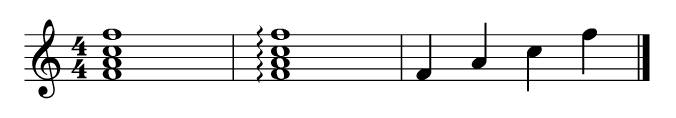
\includegraphics[width=0.8\textwidth]{expanded_major}
\caption{writeme}
\label{fig:expanded_major}
\end{figure}

On the other hand, as shown in Figure \ref{fig:nonchord_tones}, the simultaneous sounding of different notes does not necessarily give rise to the perception of different chords.
Here, a major triad is sustained under the first several degrees of its scale.
While three notes in the upper voice are contained in the C-major triad, the others --the D, F, and A-- are referred to as ``nonchord'' tones.
These extra notes are explained away in the overall harmonic scene, as they fall on metrically weak beats, are comparatively short in duration, and quickly move to notes that \emph{are} in the chord.
These embellishments do not contribute to the harmonic center of the phrase, and the bar can still be understood as a stable C-major chord.

\begin{figure}[t]
\centering
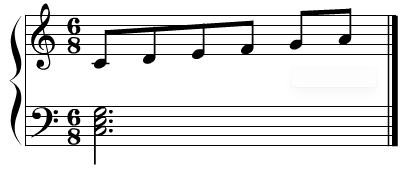
\includegraphics[width=0.8\textwidth]{nonchord_tones}
\caption{writeme}
\label{fig:nonchord_tones}
\end{figure}

A last example, shown in Figure \ref{fig:mthomework}, demonstrates the level of complexity and inherent subjectivity that may arise in the process of describing real music with chords.
Referred to as \emph{harmonic analysis}, this exercise is performed in an effort to understand the harmonic content in a theoretical manner.
Here, an excerpt of a score has been analyzed, with chords notated under the original parts.
Even in this instance, where the individual is able to operate directly on the symbolic representation, it is common to find alternate interpretations of the same musical content.
Conversely, annotations resulting from sound recordings, as opposed to a score, are referred to as \emph{chord transcriptions}.
Often the recording itself is the only musical artifact to consider, introducing even more room for subjectivity.

\begin{figure}[t]
\centering
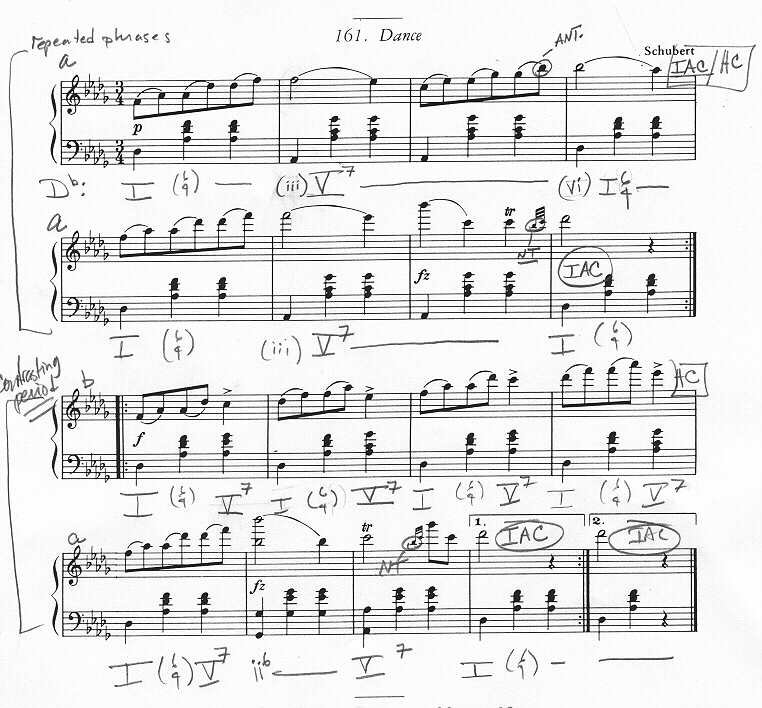
\includegraphics[width=0.8\textwidth]{practicekey2.jpg}
\caption{A sample harmonic analysis, performed as a music theory exercise.}
\label{fig:mthomework}
\end{figure}


% Skilled musicans are quite robust in the ability to assign chord labels to musical scenes despite an occasionally opaque decision making process, and it is an exciting challenge to produce a computational system with a similar capacity.


\subsection{Chord Syntax}
\label{sec:chord_syntax}

It is a pragmatic, but ultimately necessary, preliminary step to define a standard syntax for compactly notating chords.
Much of the pioneering work in this space was performed by Harte \cite{Harte2010}, and many of these conventions are utilized here.
Going forward, chords expressed in this scheme are stylized with a fixed-width font, e.g. \texttt{A:min}.

Firstly, Harte's general chord notation is described by the following four-part symbolic description:

\begin{equation}
\{r\}:\{q\}(i)/\{b\}
\end{equation}

\noindent Every chord name begins with a root $r$ in the form of a pitch class, optionally modified by zero or more sharps or flats, or one of two reserved characters: \texttt{N} for the ``null'' no-chord condition, or \texttt{X} for the special case in which the musical content cannot be described harmonically.

The root is potentially followed by a quality shorthand, $q$, separated by a colon and implying a particular set of note intervals.
Though there are a large number of possible chord qualities, this is often limited to a particular subset in practice.
Those considered in this work are indicated in the following table:

\begin{table}[h]
\begin{center}
\caption{Chord quality names and corresponding relative semitones.}
\label{tab:qualities}
\begin{tabular}{l | c | c}
Name & Shorthand & Semitones \\
\hline
Major & \texttt{maj} & $\{0, 4, 7\}$ \\
Minor & \texttt{min} & $\{0, 3, 7\}$ \\
Major 7 & \texttt{maj7} & $\{0, 4, 7, 11\}$ \\
Minor 7 & \texttt{min7} & $\{0, 3, 7, 10\}$ \\
Dominant 7 & \texttt{7} & $\{0, 4, 7, 10\}$ \\
Major 6 & \texttt{maj6} & $\{0, 4, 7, 9\}$ \\
Minor 6 & \texttt{min6} & $\{0, 3, 7, 9\}$ \\
Diminished & \texttt{dim} & $\{0, 3, 6\}$ \\
Augmented & \texttt{aug} & $\{0, 4, 8\}$ \\
Suspended 2$^{nd}$ & \texttt{sus2} & $\{0, 2, 7\}$ \\
Suspended 4$^{th}$ & \texttt{sus4} & $\{0, 5, 7\}$ \\
Fully-diminished 7 & \texttt{dim7} & $\{0, 3, 6, 9\}$ \\
Half-diminished 7 & \texttt{hdim7} & $\{0, 3, 6, 10\}$ \\
\hline
\end{tabular}
\end{center}
\end{table}


The third field provides an interval set, $i$, wrapped by parentheses.
In practice, there are two reasons for representing information intervallically.
One such instance is, through a combination of additional degrees and asterisks, the modification of a quality shorthand in order to represent a non-standard, but related, chord.
An example of this might be the chord name \texttt{A:min(\*b3, b7)}, which means that the minor third ($C$) is absent, but a minor 7 ($G$) has been added.
The other instance occurs when the intervals are certain but the spelling is ambiguous, such as \texttt{C:(1, 5)}. %; note that this is a valid spelling of the chord shown in Figure \ref{fig:powerchord_context}.

The final field of this chord syntax is the bass interval, $b$, which indicates the scale degree at the bottom of the chord.
Typically this is also the root of the chord, and is implied as such in the absence of an explicit bass interval.
However, it is necessary to state that the scale degrees of the chord --given by the quality shorthand and the interval set-- can be further augmented by the inclusion of a bass interval.
For example, the chords \texttt{C:maj/b7} and \texttt{C:7} would be understood as containing the same pitch classes, but are spelled differently.


\subsection{Motivation}
\label{subsec:motivation}

% Historical Context
Even from the earliest efforts in content-based music informatics research, automatic music transcription has stood as one of the Holy Grails of the field.
Over time, however, it would prove exceptionally difficult, and fracture into a variety of smaller, and hopefully more manageable, subtopics.
As a result, automatic chord estimation materialized as one such task, now receiving healthy attention for more than a decade, and established as a benchmark challenge at the annual MIReX event \footnote{{http://www.music-ir.org/mirex/wiki/MIREX\_HOME}}.

% Applications
% - People
Given the prerequisite skill necessary to produce these transcriptions manually, there is considerable motivation to develop automated systems capable of reliably performing this task.
As evidenced by large online communities surrounding websites like e-chords\footnote{http://www.e-chords.com} or Ultimate Guitar\footnote{http://www.ultimate-guitar.com}, countless individuals invest considerable time and effort in the curation and consumption of popular music transcriptions.
Often this is driven by desire to learn and perform music for which symbolic notation does not exist.
Conversely, automatic chord transcription systems would be particularly useful in the areas of composition, recording, and production.
Furthermore, the curation of this content would enable large-scale musicological analysis of contemporary music.

% MIR Systems
In addition to the concerns of individual users, computational systems capable of reliable chord transcription are directly useful inside the domain of content-based MIR.
Chords can serve as a robust mid-level representation with which to build systems and extract higher level musical knowledge.
This has been used in the space of cover song retrieval \cite{Juan?}, navigating large collections \cite{alan?}, and genre recognition \cite{anglade}.
Such systems would also facilitate data collection for other tasks, aiding in visualization and other facets of music transcription.

% Theoretical merit
From a more philosophical perspective, the identification of chords is also intriguing as an intelligent musical behavior, being a high level cognitive process that is often open to multiple interpretations between knowledgable experts.
Experiential bias of the annotator may manifest in the subjective decisions made by an observer, where a pianist may arrive at a different harmonic analysis than that of a guitarist due to how a collection of notes might be produced.
Lastly, the knowledge and skill of the one recognizing chords in music will affect the resulting interpretations.
Beginners will likely prefer simple or more common descriptions, whereas experts will be more aware of complex nuances and have better command over a larger harmonic vocabulary.


\subsection{Limitations}
\label{subsec:limitations}

% Limitations
It should be acknowledged that such an inquiry is subject to certain limitations, and there are several that should be discussed.
% Scope of music considered
First and foremost, this work is primarily interested in the tradition of tonal Western music, with a particular focus on popular contemporary music from the last century, in 12-TET.
% Historical context -> Harmonic analysis
Within this large body of content, the use of harmony and the language of chords has steadily evolved over time.
Contextualizing briefly, music theorists have long sought to characterize musical works via analysis and reduction as a means to understanding.
With sound recording being a relatively modern invention on the timescale of music history, much effort to this end has been invested in the analysis of symbolic notation, or scores.
From the counterpoint of J. S. Bach to the functional analysis of Heinrich Schenker or more recently Fred Lehrdal, traditional musical analysis revolves heavily around the harmonic facets of a musical piece by marginalizing the dimensions of rhythm and timbre.
As a result, the harmonic language of ``chords'' developed as an expressive, yet compact, vocabulary with which one might describe a piece of music harmonically.
Western pop music, however, is not wont to consider the rules of conventional tonal theory or compose by traditional means.
Therefore efforts to understand the former in the language of the latter is ultimately limited by the validity of this applied knowledge.

% -- previous blurb--
%  still good, but redundant?
% -------------------
% The last notable limitation is related to the validity and relevance of chords as a means to describe musical content.
% Even in the constrained space of Western tonal music set forth here, not all musical works will be well-described by the language of harmonic analysis, and thus chords may be a clumsy language with which to describe such music.
% In some cases an alternative approach to analysis, such as voice leading, might make more sense; in others, such as rap or math rock, a lack of clearly structured harmonic content may arguably render the goal of harmonic analysis altogether irrelevant.
% As a result, the application of, or conclusions resulting from, this inquiry can only be considered valid within this scope.

This realization encourages due consideration of the philosophical limits of objective truth in an inherently subjective task.
As outlined previously, the definition of a chord is open to interpretation, and one's understanding of a harmonic phrase may be influenced by individual experience, degree of skill, and intended purpose.
Furthermore, the methodology of using ``expert'' annotations in the development and evaluation of computational systems is based on the assumption that all experts share one perspective.


\section{Previous Efforts in Automatic Chord Estimation}
\label{sec:background}

% TODO: This is paltry....
This section attempts to develop a formal defintion of the automatic chord estimation task, and detail the standard methodology used by the research community.
It closes with a brief survey of the state of the art and the apparent trajectory of the research topic.


\subsection{Problem Formulation}
\label{subsec:problem_formulation}

% Problem formulation
Consistent with the motivations outlined in \ref{subsec:motivation}, the goal of an automatic chord estimation (ACE) system is --or, at least, has been-- to produce an objectively ``good'' time-aligned sequence of chords from a given music signal.
This established notion of objectivity is crucial to how the problem is approached, whereby conventional methodolgy prefers repeatable, quantitative evaluation as a proxy to qualitative feedback collected from human subjects.
While the latter is generally preferable to the former, such user studies can be prohibitively costly in both time and money to conduct with any regularity.
As a result, the research of computational systems that model human behavior often proceeds by collecting some number of input-output datapoints from human subjects \emph{beforehand}, and subsequently measuring the degree to which a system can produce these outputs from the inputs.
Importantly, this paradigm operates on the assumption that these human provided input-output pairs, conventionally referred to as ``ground truth'' in various domains, are absolute, and not a function subject.

% Datasets and human annotations
The first major effort to curate ground truth chord transcriptions was led by Harte in the mid-2000s \cite{Isophonics}, where a small team of individuals transcribed the entire discography of The Beatles.
Containing chord annotations for 180 tracks, this was a landmark dataset in the field of MIR and shaped years of ACE research.
More recently, two datasets were made publicly available following the 2011 Conference of the International Society of Music Information Retrieval (ISMIR), one of over 700 tracks led by J. Ashley Burgoyne \cite{Burgoyne2011} and another of 295 tracks led by Tae Min Cho \cite{Cho2011b}; for convenience, we will refer to the former as ``Billboard'' and the latter as ``NYU'', corresponding to the related projects.
Along the way, one additional, comparatively small, dataset was released, containing 20 tracks by the band Queen, provided by Matthias Mauch \cite{Mauch2009x}.
In all four cases, the chord transcriptions are provided on the premise that the data corresponds to the ``expert'' perspective.
To prevent errors or resolve judgment calls, all annotation efforts named above employed a review process, where the transcriptions of one or more annotator were verified by a different individual.

% Transcription, estimation and recognition
% Somewhat ironically, there is some inconsistency in the literature regarding what this task should be called.
% Mauch makes mention of this in his thesis \cite{Mauch2010PhD},

% The issue of vocabularies -- Major-minor Chord mapping
As we have seen in \ref{subsec:foundations}, it is a particular nuance of chord naming conventions that the vocabulary of possible chord names is effectively infinite.
This results in a few practical problems that must be resolved.
While the majority of musical content will be well described by a bounded subset of chord spellings, a large number of low-frequency chord names will naturally occur in a dataset.
This is made worse by the reality that some chord qualities, namely \texttt{maj} or \texttt{min}, are simply more common than the rest.
Taken together, chord estimation systems are typically designed to classify chords among a fixed vocabulary defined \emph{a priori}.

In the history of ACE, the choice of vocabulary has been anything but standard, influenced by a variety of factors.
Data-driven approaches, for example, can be sensitive to the amount of labeled data available to train a given model, in which case it might be advantageous to discard under-represented chord classes.
Alternatively, it might be a useful constraint of the system to only predict the most common chords, helping to cut down on confusions and spurious errors, or perhaps a researcher is not particularly interested in detecting inversions.
It therefore becomes equally challenging to compare the performance of systems designed for different vocabularies.

One common strategy devised by the community to cope with this variation is the concept of Major-Minor chord resolution.
This proceeds by taking the space of all chord names in a collection of transcribed music recordings, and mapping each chord name to either a Major or Minor chord with the same root \cite{McVicar2013}.
Though some chord quality resolutions are musically reasonable, e.g. \texttt{maj7} $\to$ \texttt{maj}, others are less sound, e.g. \texttt{dim7} $\to$ \texttt{min} or \texttt{aug} $\to$ \texttt{maj}.
A thorough discussion on the impacts of such decisions will take place in Section \ref{sec:pilot_study}, but we address the practice of \emph{vocabulary resolution} here to call attention to the fact that, save for a few exceptions, the majority of ACE research and methodology focuses on this artificial Major-Minor formulation.


\subsection{Computational Approaches}
\label{subsec:computational_approaches}

% Previous work
Historically speaking, nearly all approaches to the ACE task adopt the same basic architecture, diagrammed in Figure \ref{fig:basic_ace}.
First, harmonic features, referred to as pitch class profiles (PCP) or \emph{chroma}, are extracted from short-time observations of the audio signal.
Initially proposed for use in chord estimation systems by Fujishima \cite{fujishima1999}, chroma features attempt to measure the amount of energy in the signal corresponding to the 12 pitch classes named in Eq. \ref{eq:pitch_classes}.
These features may then be processed by any number of means, referred to in the literature as \emph{pre-filtering}.
Importantly, this is done prior to the next stage of \emph{pattern matching}, which is performed on the final feature representation to measure how similar the observed signal is to a set of chord names.
The process of pattern matching, a relatively local operation, is mapped over a much longer signal, e.g. a full recording, yielding a time-varying estimate of the various chord types the model can represent.
Finally, \emph{post-filtering} is applied to the output of the pattern matching stage, resulting in a sequence of chord names over time.

Though the implementation details have continued to evolve over the last decade, the brunt of chord estimation research has concentrated not on the fundamental system per se, but rather the tuning of its components.
In particular, much time and energy has been invested in developing not just better features, but specifically better \emph{chroma} features \cite{muller2010}.
Complementing chroma features, others have explored the use of multi-band chroma to model bass frequencies separately \cite{Mauch2009?} or a Tonnetz representation in an effort to better encode harmonic relationships between chords \cite{Lee2007}.
Acknowledging the challenges inherent to designing good features, Pachet et al pioneered work in automatic feature optimization \cite{pachet2004}, and more recently deep learning methods have been employed to learn robust Tonnetz features \cite{ejh2011}.
Early methods focused on local smoothing, such as low-pass \cite{} or median \cite{} filtering as a form of pre-filtering, but more recently some methods have attempted to leverage the repeated nature of music to yield more stable estimates of the harmonic composition at a given point in time \cite{Cho2011}.
Various classification strategies have been investigated such as binary templates \cite{?}, Dirichlet distribution models \cite{Burgoyne2008?}, or Support Vector Machines (SVMs) \cite{weller2009}, but Gaussian Mixture Models (GMM) are by and large the most common feature modeling approach \cite{a,b,c}.
The choice of post-filtering methods has been shown to significantly impact system performance, and much research has focused on properly tuning Hidden Markov Models (HMMs) \cite{Cho2010}, first introduced by \cite{sheh2003}.
Recently, in an effort to continue to advance the state of the art, researchers have begun exploring more complex post-filtering methods such as Dynamic Bayesian Networks (DBNs) \cite{mauch2010b, McVicar2013} and Conditional Random Fields (CRFs) \cite{?}.

It is worth noting that in this lineage, the systems that do make use of data-driven learning typically only do so in disjoint stages.
More often than not, machine learning is only performed at the pattern matching stage, where increasingly powerful models are fit to hand-crafted features.
A few works do attempt to learn features, such as \cite{MauchNNLS, Humphrey2012?}, but the different stages are optimized independetly.
Though it is standard practice to train a GMM/HMM jointly, some have observed that learning the parameters of the HMM, i.e. the transition probabilities, yields no significant benefit over a uniform probabilities with a strong self-transition affinity \cite{Cho2014PhD}.
One notable work that attempts to jointly optimize multiple stages is that of \cite{Kim2012}, which optimizes the GMM to a minimum classification error (MCE), rather than a conventional maximum likelihood formulation.


\subsection{Evaluation Metrics}
\label{subsec:evaluation_metrics}

We now formalize an approach to comparing, and subsequently scoring, the relative agreement between two chord transcriptions.
The classic metric reported in ACE research is conceptually some kind of total mutual agreement score, $S$, between a set of $N$ reference, $\mathcal{R}$, and estimated, $\mathcal{E}$, transcriptions as a continuous integral over time, defined by the following:

\begin{equation}
S_overall = \frac{1}{W}\sum_{n=0}^{N-1}\int_{t=0}^{T_n}C(\mathcal{R}_n(t), \mathcal{E}_n(t))\partial~t
\end{equation}

\noindent where $C$ is a chord comparison function, $t$ is time, $n$ the index of the track in a collection, $T_n$ the duration of the $n^{th}$ track, $W$ the cumulative amount of time on which $C$ is defined.
More explicitly, $W$ is computed by a similar integral:

\begin{equation}
W = \sum_{n=0}^{N-1}\int_{t=0}^{T_n}(\mathcal{R}_n(t), \mathcal{E}_n(t) \in \Re)\partial~t
\end{equation}

Defining the score normalization term $W$ separately is useful when comparing chord names, as it relaxes the assumption that the comparison function is defined for all possible chords.
Therefore vocabulary selection or resolution can be delayed until evalutation, and all emphasis can be placed on the comparison function $C$.
In practice, this measure is known as \emph{Total Correct Overlap} (TCO) \cite{Mauch, Harte, McVicar}, \emph{Weighted Chord Symbol Recall} (WCSR) \cite{MIReX}, or \emph{Framewise Recognition Rate} \cite{Cho2014}.
Effectively, this is a multiclass version of recall, which is expressed by the following:

\begin{equation}
r = \frac{true~positives}{all~positives}
\end{equation}

Precision, a complement to recall, can also be expressed similarly:

\begin{equation}
p = \frac{true~positives}{true~positives + false~positives}
\end{equation}

\noindent While the definition of recall intuitively extends to the multiclass condition faced in ACE, it is worthwhile to consider the meaning of precision.
In this instance, such a measure provides insight into how reliable the estimated chord name are.
For example, a system could heavily over-predict the most common chord labels to achieve a high recall value, but the precision might still be comparatively low.
% Notably, if the errors (false positives) are decorrelated, then recall and precision will converge to the same value.
Standard practice in information retrieval also considers the harmonic mean of these two metrics, known as the $f_1$ score, which captures both behaviors in a single measure:

\begin{equation}
f_1 = \frac{pr}{2(p+r)}
\end{equation}

Finally, it was recently proposed by Cho in \cite{Cho2014PhD} that, when working with larger chord vocabularies, special attention should be paid to performance across all chord qualities.
The motivation for additional measures stems from the reality that chord classes are not uniformly distributed, and a model that ignores infrequent chords will not be well characterized by global statistics.
This can be extended to the metrics above by adding a quality condition to the comparison function and averaging over qualities:

\begin{equation}
S_{quality\_ave} = \sum_{q=0}^{Q-1}\frac{1}{W_q}\sum_{n=0}^{N-1}\int_{t=0}^{T_n}C(\mathcal{R}_n(t), \mathcal{E}_n(t) | q)\partial~t
\end{equation}

\noindent Referred to as \emph{Average Chord Quality Accuracy} (ACQA), this is simply a recall measure where the contributions of the individual chord qualities are reweighted.
Though it was not addressed at the time, this approach to quality-wise evaluation can be mapped to precision and $f_{1}$, providing a more complete set of metrics with which to better understand the behavior of a system.


% Data collection
\section{Pilot Study}
\label{sec:pilot_study}

Here, we revisit the work of a preliminary study conducted by the author in 2012, and presented at the International Conference of Machine Learning and Applications (ICMLA 2012) \cite{Humphrey2012}.
Approaching ACE from the perspective of classifying music audio among the standard 24 Major-Minor classes, in addition to a no-chord estimator, a deep convolutional network is explored as a means to realize a full chord estimation system.
Doing so not only alleviates the questions of relevance or quality toward chroma as a representation, but error analysis of an end-to-end data-driven approach can be used to gain insight into the data itself.
In this section, the brief analysis provided in the original publication is expanded in greater detail.


\subsection{Research Questions}
\label{subsec:research_questions}

Even in the instances of previous work that jointly optimize different processing stages, the systems are bottlenecked by the choice of feature representation, e.g. chroma.
As a result, it is unclear which stage is most responsible for unsatisfactory performance, and history indicates most believe more powerful classifiers will lead to better results.
Meanwhile, it has been demonstrated in other disciplines that deep learning can be used to build extremely complex models, at which point it can be trivial to overfit the data used for training.
Though often seen as a detriment or challenge, it is seen here as a opportunity to better understanding of the problem, giving rise to two related questions: one, how does performance change as a function of model complexity, and two, in what instances can the model \emph{not} overfit the training data?
Additionally, how can domain knowledge be used to inform the application of a deep learning to the estimation of chords from audio?


\subsection{Experimental Setup}
\label{subsec:experimental_setup}

% Input Representations
Audio signals are downsampled to 7040Hz and transformed to a constant-Q time-frequency representation, described previously in \ref{chp:constant_q}.
This transform consists of 36 bins per octave, resulting in 252 filters spanning 27.5--1760Hz, and is applied at a framerate of 40Hz.
The high time-resolution of the constant-Q spectra is further reduced to a framerate of 4Hz by mean-filtering each frequency coefficient with a 15-point window and decimating in time by a factor of 10.
As discusseed, a constant-Q filterbank front-end provides the dual benefits of a reduced input dimensionality, compared to the raw audio signal, and produces a time-frequency representation that is linear in pitch, allowing for convolutions to learn pitch-invariant features.
It is also worth noting that this filterbank front-end can be interpreted as hard-coding the first layer of a larger convolutional architecture.

The input to the network is defined as a 20-frame time-frequency \emph{patch}, corresponding to 5 seconds.
A long input duration is chosen in an effort to learn context, thereby reducing the need for post-filtering.
Additionally, the application of local-contrast normalization is considered as an experimental variable, as defined in \ref{chp:deep_learning}.
This pre-processing of the constant-Q representation serves as a form of automatic gain control, and somewhat similar in principle to log-whitening used previously in chord estimation \cite{Cho2011}.
During training, we also consider the application of random shifts of the data in frequency as a data augmentation.
The linearity of pitch in a constant-Q representation affords the ability to ``transpose'' an observation as if it were a true data point in a different pitch class by shifting the pitch tile and changing the label accordingly.
Every data point in the training set then counts toward each chord class of the same quality (Major or minor), effectively increasing the amount of training data by a factor of 12.

% Architectures
A five-layer 3D convolutional network, as defined in \ref{chp:deep_learning}, is taken as the general model, consisting of three convolutional layers and two fully-connected layers; a diagram is provided in Figure \ref{fig:chordnet_take1}.
Six different model complexities are explored by considering two high-level variables: the width of each layer, as the number of kernels or units, and the shape of the receptive fields.
A table of these configurations are given in Table \ref{tab:model_configs}, and an index tuple notation is adopted to compactly reference the different models.
Note that only the first convolutional layer makes use of pooling, and only in the frequency dimension, by a factor of three in an effort to learn slight intonation invariance.
The output of the final layer is passed through a softmax operator, given previously by \ref{eq:softmax}, producing an output that behaves like a probability mass function over the chord classes.


\begin{table}[!t]
% increase table row spacing, adjust to taste
\renewcommand{\arraystretch}{1.4}
% if using array.sty, it might be a good idea to tweak the value of
% \extrarowheight as needed to properly center the text within the cells
\caption{Model Configurations - Higher indices correspond to a larger number of parameters.}
%\caption{Convolutional Layers -- K: kernel shape, P: pooling shape. Fully-connected Layers -- W: Weight shape }
\label{table:model_configs}
\centering
% Some packages, such as MDW tools, offer better commands for making tables
% than the plain LaTeX2e tabular which is used here.
\begin{tabular}{c || l || l |}
 & --1 & --2 \\
\hline
 1 & K:(1, 4, 6, 25), P:(1, 3)& K:(1, 4, 5, 25), P:(1, 3)\\
 &K:(4, 6, 6, 27) & K:(4, 6, 5, 13) \\
 &K:(6, 8, 6, 27) & K:(6, 8, 5, 13) \\
 &W:(480, 50)  & W:(2560, 50)\\
 &W:(50, 25)  & W:(50, 25)\\
\hline
 2 & K:(1, 6, 6, 25), P:(1, 3)& K:(1, 6, 5, 25), P:(1, 3)\\
 &K:(6, 9, 6, 27) & K:(6, 9, 5, 13) \\
 &K:(9, 12, 6, 27) & K:(9, 12, 5, 13) \\
 &W:(720, 125)  & W:(3840, 125)\\
 &W:(125, 25)  & W:(125, 25)\\
\hline
 3 & K:(1, 16, 6, 25), P:(1, 3)& K:(1, 16, 5, 25), P:(1, 3)\\
 &K:(16, 20, 6, 27) & K:(16, 20, 5, 13) \\
 &K:(20, 24, 6, 27) & K:(20, 24, 5, 13) \\
 &W:(1440, 200)  & W:(7680, 200)\\
 &W:(200, 25)  & W:(200, 25)\\
\hline
\end{tabular}
\end{table}


% Training
As this work predates access to the Billboard and Queen datasets, only the NYU and Beatles collections are considered, totalling 475 tracks.
All chord names are resolved to their nearest major-minor equivalent, as discussed in \ref{subsec:problem_formulation}, based on the third scale degree: \texttt{min} if the quality should contain a flat third, otherwise \texttt{maj}.
The collection of 475 tracks are stratified into five folds, with the data being split into training, validation, and test sets at a ratio of 3--1--1, respectively.
The algorithm by which the data are stratified is non-trivial, but somewhat irrelevant to the discussion here; we refer the curious reader to the original publication for more detail.
Model parameters are learned by minimizing the Negative Log-Likelihood (NLL) loss over the training set.
This is achieved via mini-batch stochastic gradient descent with a fixed learning rate and batch size, and early stopping is performed as a function of classification error over the validation set.
Training batches are assembled by a forced uniform sampling over the data, such that each class occurs with equal probability.
All experiments are cross validated five times such that each fold is used as the test set once.


\subsection{Quantitative Results}
\label{subsec:quantitative_results}

Following the discussion of evaluation in \ref{subsec:evaluation}, it is sufficient to define a simple equivalence matching function for comparing two chord names, as all chords in the dataset have been resolved to one of the 24 major-minor:

\begin{displaymath}
   C(x, y) = \left\{
     \begin{array}{lr}
       1.0 & x == y \\
       0.0 & otherwise
     \end{array}
   \right.
\end{displaymath}

\noindent Furthermore, at this stage of research, the only metric considered is that of overall recall, and all performance statistics given here correspond to this measure.


\begin{table}[!t]
% increase table row spacing, adjust to taste
% \renewcommand{\arraystretch}{1.4}
% if using array.sty, it might be a good idea to tweak the value of
% \extrarowheight as needed to properly center the text within the cells
\caption{Overall recall for two models, with transposition and LCN.}
\label{table:exp1res}
\centering
% Some packages, such as MDW tools, offer better commands for making tables
% than the plain LaTeX2e tabular which is used here.
\begin{tabular}{c || c c c || c c c |}
 & & Arch 3--1 & & & Arch 1--1 & \\
 \hline
Fold & Train & Valid & Test & Train & Valid & Test \\
\hline
1 & 83.2 & 77.6 & 77.8 &  79.6 & 76.9 & 76.8 \\
2 & 83.6 & 78.2 & 76.9 & 80.5 & 77.0 & 76.8 \\
3 & 82.0 & 78.1 & 78.3 & 80.0 & 77.2 & 78.2\\
4 & 83.6 & 78.6 & 76.8 & 80.2 & 78.0 & 75.8 \\
5 & 81.7 & 76.5 & 77.7 & 79.5 & 75.9 & 76.8 \\
\hline
Total &  82.81 & 77.80 & \textbf{77.48} & 79.97 & 77.00 & \textbf{76.87}\\
\hline
\end{tabular}
\end{table}

As an initial benchmark, it is necessary to consider performance variance over different test sets.
We are less interested in absolute performance than general trends, and evaluating all model complexities over all folds is unnecessary if the performance is reasonbly stable.
The outer model configurations in the first column of Table \ref{tab:model_configs} (Arch:3--1 and Arch:1--1) were selected for five-fold evaluation, influenced by run-time considerations.
Overall recall is given in Table \ref{table:exp1res}, and offers two important insights.
One, deep network chord estimation performs competitively with the state of the art at the major-minor task.
Previously published numbers on the same dataset fall in the upper 70\% range \cite{Cho2011}, and it is encouraging that this initial inquiry can roughly match the performance resulting from more than a decade of research.
More importantly for our purposes here, variation in performance falls within a 2\% margin.

Given the stability of performance across folds, we can confidently explore the other model complexities with a leave-one-out (LoO) strategy.
Noting that training and validation performance are lowest for the fifth fold, we select this split of the data for training across configurations with and without data augmentation.
We base this decision on the premise that this particular split of the data provides the greatest opportunity for error analysis.

The overall recall results are given in Table \ref{table:sweep}.
Perhaps the most immediately noticeable trend is the differential in recall on the training set between data conditions.
Transposing the training data improves generalization, in addition to reducing the extent to which the network can overfit the training data.
Transposing the input pitch spectra should have a negligible effect on the parameters of the convolutional layers, and this is exactly what occurs in the model.
All models in the second column, e.g. X-2, have smaller kernels, which leads to a much larger weight matrix in the first fully connected layer, and worse generalization in the non-transposed condition.
It is reasonable to conclude that over-fitting mostly occurs in the final layers of the network, which do not take advantage of weight tying.
Transposing the data results in an effect similar to that of weight tying, but because the sharing is not explicit the model must learn to encode this redundant information.


\begin{table}[!t]
% increase table row spacing, adjust to taste
% \renewcommand{\arraystretch}{1.4}
% if using array.sty, it might be a good idea to tweak the value of
% \extrarowheight as needed to properly center the text within the cells
\caption{Performance as a function of model complexity, over a single fold.}
\label{table:exp2res}
\centering
\begin{tabular}{ c || c c c || c c c |}
& & As-Is & & & Transposed & \\
 \hline
Arch & Train & Valid & Test & Train & Valid & Test \\
\hline
1-1 & 84.7 & 74.9 & 75.6 & 79.5 & 75.9 & 76.8 \\
2-1 & 85.5 & 75.0 & 75.5 & 80.6 & 75.6 & 77.0 \\
3-1 & 92.0 & 75.2 & 75.5 & 81.7 & 76.5 & 77.7 \\
\hline
1-2 & 87.0 & 73.1 & 74.5 & 78.4 & 75.5 & 76.2 \\
2-2 & 91.2 & 73.9 & 74.0 & 79.4 & 75.4 & 76.6 \\
3-2 & 91.7 & 73.6 & 73.8 & 81.6 & 76.3 & 77.4 \\
\hline
\end{tabular}
\end{table}


\subsection{Qualitative Analysis}
\label{subsec:Qualitative_analysis}

While the quantitative results obtained in the previous discussion are certainly encouraging, we have yet to fully address the larger research objectives.
As indicated by Table \ref{tab:exp2res}, transposing the data during training slightly improves generalization, but more so limits the degree to which the models can overfit.
It is important to recognize that these behaviors are not necessarily linked, and therefore whatever these networks learn as a result of data augmentation is preventing it from overfitting a considerable portion of the training set.


\begin{figure}[!t]
\centering
 \centerline{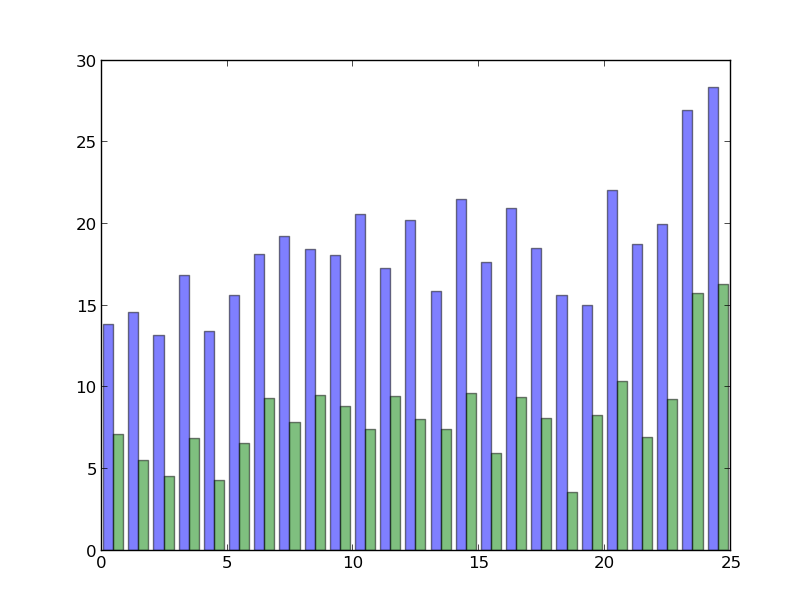
\includegraphics[width=5in]{tr-te-diff_FF-TT}}
\caption{Accuracy differential between training and test as a function of chord class, ordered along the x-axis from most to least common in the dataset for ETD:False (blue) and ETD:True (green) conditions.}
\label{fig:classes}
\end{figure}

One potential cause of over-fitting is due to an under-representation of some chord classes in the dataset.
If this were the case, we would see the most frequent classes unaffected by data augmentation, while less common classes would exhibit drastic swings in performance.
Focusing here on Arch:3--1, Figure \ref{fig:classes} shows the change in accuracy between data conditions for both training and test sets as a function of chord class, sorted by most to least common in the dataset.
This plot indicates that, while transposing data during training reduces over-fitting, it does so uniformly across chord classes, on the order of about $10\%$.
Therefore, all chord classes benefit equally from data augmentation, which is characteristic of intra-class variance more so than inadequate data for less common classes.

\begin{figure}[!t]
\centering
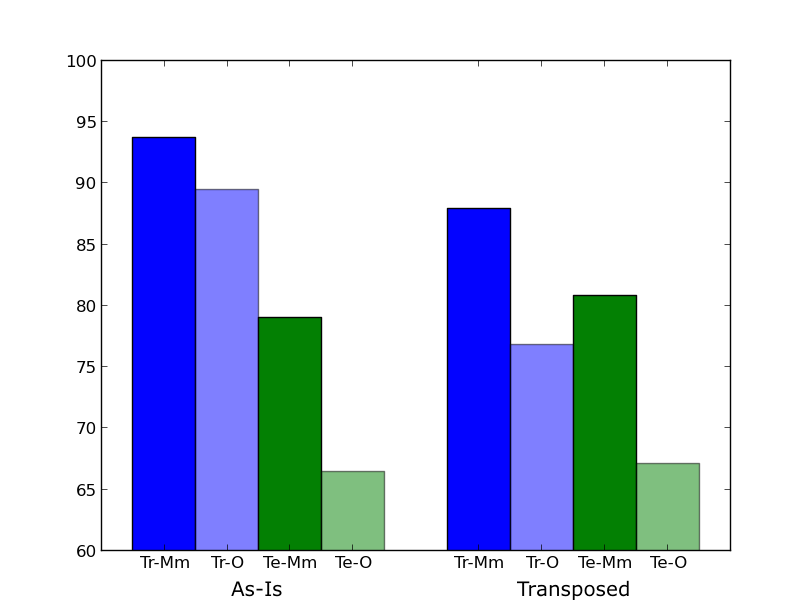
\includegraphics[width=5in]{FF-TT_Mm-vs-other}
\caption{Effects of transposition on recognition accuracy as a function explicitly labeled Major-Minor chords (dark bars), versus other chord types (lighter bars) that have been resolved to their nearest Major-Minor equivalent, for training (blue) and test (green) in standard (left) and transposed (right) conditions.}
\label{fig:strict_vs_others}
\end{figure}

If this is indeed the case, there are likely two main sources of intra-class variance: the practice of resolving all chord classes to Major-Minor, or error in the ground truth transcriptions.
As a means to assess the former, Figure \ref{fig:strict_vs_others} plots the accuracy for chords that strictly labeled root-position Major-minor (Mm) versus all other (O) chords that are mapped into these classes in the train (Tr) and test (Te) conditions, with and without transposition.
This is a far more informative figure, resulting in a few valuable insights.
First, there is a moderate drop in performance over the training set for strictly Major-minor chords when data are transposed ($\approx -5\%$), but this causes a noticeable increase in generalization for strictly Major-minor chords in test set ($\approx +3\%$).
Other chords, however, experience a significant decrease in performance within the training set ($\approx -11\%$) with transposition, but register a negligible improvement in the test set ($>1\%$).
One interpretation of this behavior is there is too much conceptual variation in the space of Other chords to meaningfully generalize to unseen data that is also not strictly Major-minor.
This defintion by exclusion gives rise to a class subset that is less populated than its strict counterpart, but will inherently contain a wider range of musical content.
Though a sufficiently complex model may be able to overfit these datapoints in the absence of transposition, counting each observation toward every pitch class distributes the added variance across all classes evenly.
This causes the model to ignore the most uncommon class ``modes'' as noise, while reinforcing the strict Major-minor model in the process.

% Additionally, not only is generalization for strict Major-minor chords considerably better than that of Other chords when trained with transposition, but it achieves better recall than Other chords in the training set.
% This means ...

\begin{figure}[!t]
\centering
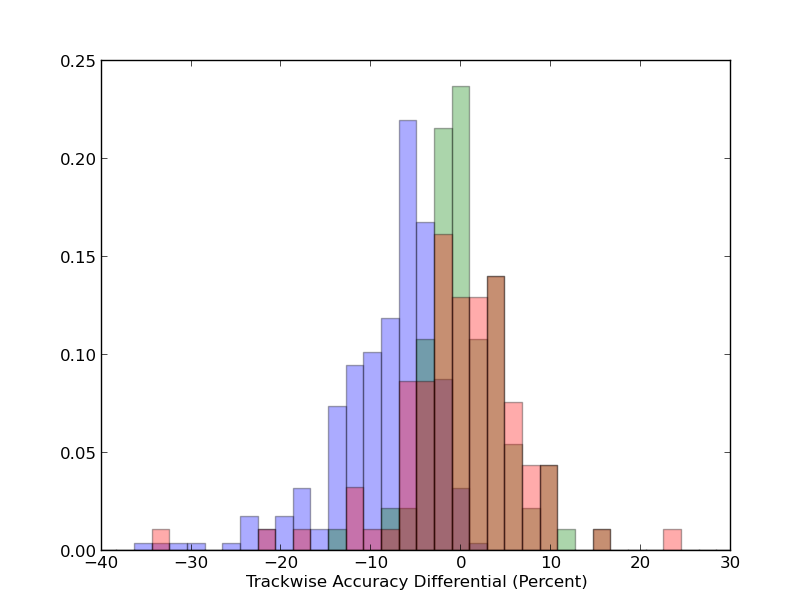
\includegraphics[width=5in]{arch_5-FF_TT_accdiff2}
\caption{Histograms of trackwise recall differential between normal and transposed data conditions, for training (blue), validation (red) and test (green) datasets.}
\label{fig:acc_diff}
\end{figure}

In addition to the effects of vocabulary resolution, there is also a question where this error resides in the data.
To address this point, we consider track-wise histograms of recall differential before and after transposing data for the training, validation, and test splits, shown in Figure \ref{fig:acc_diff}.
Interestingly, performance over most tracks is unaffected or only slightly changed by the transposed data condition, as evidenced by the near-zero mode of the distributions.
Some tracks in the training set, however, result in considerably worse performance when the data is transposed.
This is intuitively satisfying because the repetitive nature of music would cause observations drawn from the same recording to be highly correlated, and therefore multiple instances of rare chords, outliers, or labeling errors should be well localized.
Additionally, this clearly indicates that some tracks are particularly challenging or problematic, and may offer insight into future areas of improvement.

\begin{figure}[!t]
\centering
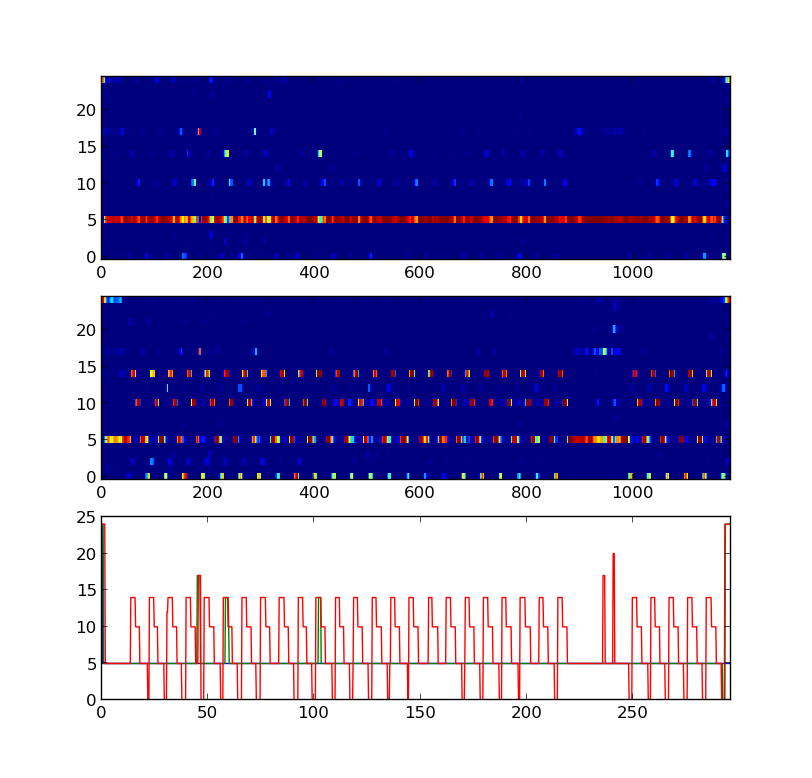
\includegraphics[width=5in]{u2-ff_tt_gtplot}
\caption{.}
\label{fig:u2fu}
\end{figure}

An instance of one such ``problem'' track, ``With or Without You'' by U2, is given in Figure \ref{fig:u2fu}.
Here, the ground truth transcription consists primarily of four chords: \texttt{D:maj}, \texttt{D:maj/5}, \texttt{D:maj6/6}, and \texttt{D:maj(4)/4}.
When resolved to the Major-minor vocabulary, the transcription is reduced entirely to \texttt{D:maj}.
Without transposing data during training, the model is able to call nearly the entire track \texttt{D:maj}; with transposition during training, however, the model is unable to reproduce the ground truth transcription and instead tracks the bass motion, producing \texttt{D:maj}, \texttt{A:maj}, \texttt{B:min}, and \texttt{G:maj}, a very common harmonic progression in popular music.
As far as quantitative evaluation is concerned, this second estimation exhibits a high degree of mismatch with the reference transcription, but is qualitatively reasonable and arguably far more useful to a musician.

\subsection{Conclusions}
\label{subsec:conclusions}

Following this initial inquiry, there are a number of conclusions to draw that should influence subsequent work.
First and foremost, the practice of chord name resolution is the largest source of error, both in training and test, as doing so creates multi-modal distributions that can be difficult to model directly.
This challenge stems from the combination of weak conceptual associations between the classes, and diminshed amount of data for the model to discover such diverse relationships.
Therefore, if for this reason alone, future work should consider larger vocabulary chord estimation, as the additional labeling information simplifies the learning problem by encouraging the machine to model different pockets of class densities separately.
Additionally, there is some evidence, in the vein of Figures \ref{fig:acc_diff} and \ref{fig:u2fu}, that chord names with modified intervals or bass information may be used inconsistently across transcriptions.
The tracks that are most affected through the use of transpostion during training are those consisting of non-standard spellings.
Seeing as how such instances comprise a relatively small portion of the data, ignoring these over-specified chord names should lead to more stable evaluation while maximizing confidence in the ground truth annotations.


\section{Large Vocabulary Chord Estimation}
\label{subsec:large_vocabulary_ace}

In light of observations resulting from the previous study, combined with other recent trends in ACE research, we now focus on the task of large vocabulary ACE.
As mentioned, there is a smaller subset of research focusing on vocabularies past the Major-minor formulation, but, for the same reasons discussed in \ref{subsec:problem_formulation}, comparing these efforts directly is problematic due to differences in vocabularies considered and the data used.

One of the most advanced large-vocabulary ACE systems to date is the recent work of Cho \cite{Cho2014}.
For context, this system design is consistent with the previous overview of ACE research, whereby the different stages of the system are modified separately.
A multiband chroma representation is computed from beat-synchronous audio analysis, producing 4 parallel chroma features.
Each is modeled by a separate Gaussian Mixture Model, yielding four separate observation likelihoods as a function of time.
These four are then decoded jointly, using a k-stream HMM, resulting in a time-aligned chord sequence.
Not only is this work one of the highest performing systems at the recent iteration of MIReX, but we are also priviledged by access to a software implementation, thereby enabling direct comparisons with other work.
It also considers a significantly larger vocabulary than previous work, and presents an even greater challenge to the application of deep learning to ACE.


\subsection{Data Considerations}
\label{subsec:data_considerations}
% Say something about Taemin's dissertation.
Following the previous work of Cho \cite{Cho2014}, we also consider thirteen chord qualities, given in Table \ref{tab:qualities} in all 12 pitch classes, plus one no-chord class, for a total of 157 classes.
Having all four datasets at our disposal, we merge these information sources into the largest collection of chord transcriptions used to date, totalling 1235 tracks.
After performing fuzzy string matching on a manifest of the known artist names and track titles, we identify X redundant tracks and randomly drop all but one from the collection; this results in a final count of 12XX tracks.

Combining conclusions from the previous section with recent discussion of evaluation at MIReX, we chose to ignore all chord instances with names that specify interval modifications, e.g. \texttt{A:min(*b3)}, or bass scale degrees that are not strictly contained by the chord shorthand, e.g. \texttt{C:maj/4}.
The decision is made in the interest of annotation consistency; considering that the cumulative data is compiled from multiple sources and several dozen annotators, it is quite unlikely that such conventions were applied identically by all subjects involved.
This subset comprises only a small percentage of the overall data ($?.?\%$), and helps filter out curious chord spellings, such as \texttt{D:maj(\*1)/$\sharp$1} or \texttt{A:maj(2,\*3)/2}.

% Statistics
Unsurprisingly, as the data is collected from real music, the distribution of absolute chord classes is extremely imbalanced.
In fact, some chord qualities do not occur in every root, and stratifying the data for training, validation, and testing only exacerbates the issue.
Much previous work, including the previous discussion, has demonstrated that chord names can be rotated to distribute instances across qualities, rather than absolute classes, motivating root-invariant analysis.
A root-invariant histogram of the chord qualities contained in the merged dataset, given in Figure \ref{fig:training_distribution}, clearly shows there is severe relative and absolute class imbalance.
To the former, a stark division exists between the majority classes (\texttt{maj}, \texttt{min}, \texttt{maj7}, \texttt{min7}, \texttt{7}, and \texttt{N}), and the minority classes (\texttt{maj6}, \texttt{min6}, \texttt{dim}, \texttt{aug}, \texttt{sus4}, \texttt{sus2}, \texttt{dim7}, \texttt{hdim7}).
The ratio, for example, between the most and least common qualities, \texttt{maj} and \texttt{dim7} respectively, is nearly three orders of magnitude ($\approx 700$).
Arguably, the more challenging imbalance is an overall lack of data for some minority classes.
Over all roots, the total duration of \texttt{dim7} is on the order of hundreds of seconds.
Considering the repetitive structure of music, it is reasonable to assume that these few instances also occur in the same small number of tracks, limiting the variability of this data.


\subsection{Research Questions}
\label{subsec:research_questions}

What can we do to overcome these issues of class imbalance?
% Build class invariance into the model
% use dropout during training
% smaller inputs, more constraints, leverage HMM for context / stabilization
How does the deep learning system compare to the state of the art?
% Beats it! depending on who you ask, at least
What are the advantages and challenges of training with larger vocabularies?
% Resolve predictions back to maj / min, how does it do? Should be better...
% Larger vocabularies result in more class collisions
% But this is actually a manifestation of ambiguity
Does observed system behavior correspond to quantitative evaluation?
% Getting a lot of reasonable confusions.
% Maybe this is a function of an inherently subjective task.
% The ground truth data on hand were ``reviewed'', and there are no records concerning which chord names may have been contested or corrected.
% Rock corpus



\subsection{Experimental Setup}
\label{subsec:experimental_setup}
This work proceeds directly from the previous study, and takes a similar approach in many facets.
There are a handful of important distinctions to make between the two, however, and these differences are detailed here.

\subsubsection{Input Representation}
\label{subsubsec:data_considerations}
A comparable constant-Q transform is applied to the audio at a framerate of 20Hz, without subsequent low-pass filtering or decimation, and time-frequency patches are formed from 20 frames, corresponding to 1 second.
Whereas the previous study aimed to learn context directly, there is the inherent concern that a low input framerate will reduce the amount of data available for training beyond what is required by the model.
In lieu of learning this context, standard post-filtering will be applied in the form of a uniform-transition HMM with a tunable self-transition penalty, consistent with \cite{Cho2014PhD}; this is introduced in greater detail shortly, in \ref{subsubsec:viterbi}.

Additionally, local contrast normalization is included as a standard preprocessing stage, with minor modifications.
In previous work, a threshold is placed on the scaling term given by the average standard deviation over the entire input.
While this may be suitable in the field of computer vision, where spatial dimensions are equivalent in 2-space, audio data behave differently in time and frequency.
Namely, complex sounds often exhibit an overtone series, and energy becomes more densely concentrated in higher frequencies.
This can have the undesirable effect of inadequately gaining regions that are more sparse.
To correct for this behavior, the scaling coefficient is adjusted such that the frequency range considered is a piecewise function of frequency height, defined as follows:

\begin{equation}
X_filt = (X \circledast W) \\
V = X_filt - X \\
S_k = V \circledast W_k \\
S_k = max(S_k, \mu_{S_k}) \\
Y = \sum_{k=0}^{K-1} g_k * \frac{V}{S_k} \\
\end{equation}

\noindent To illustrate the benefit of this piecewise combination, an example track is given in Figure \ref{lcn_mods}, both with and without the octave-dependent modification.

\begin{figure}[!t]
\centering
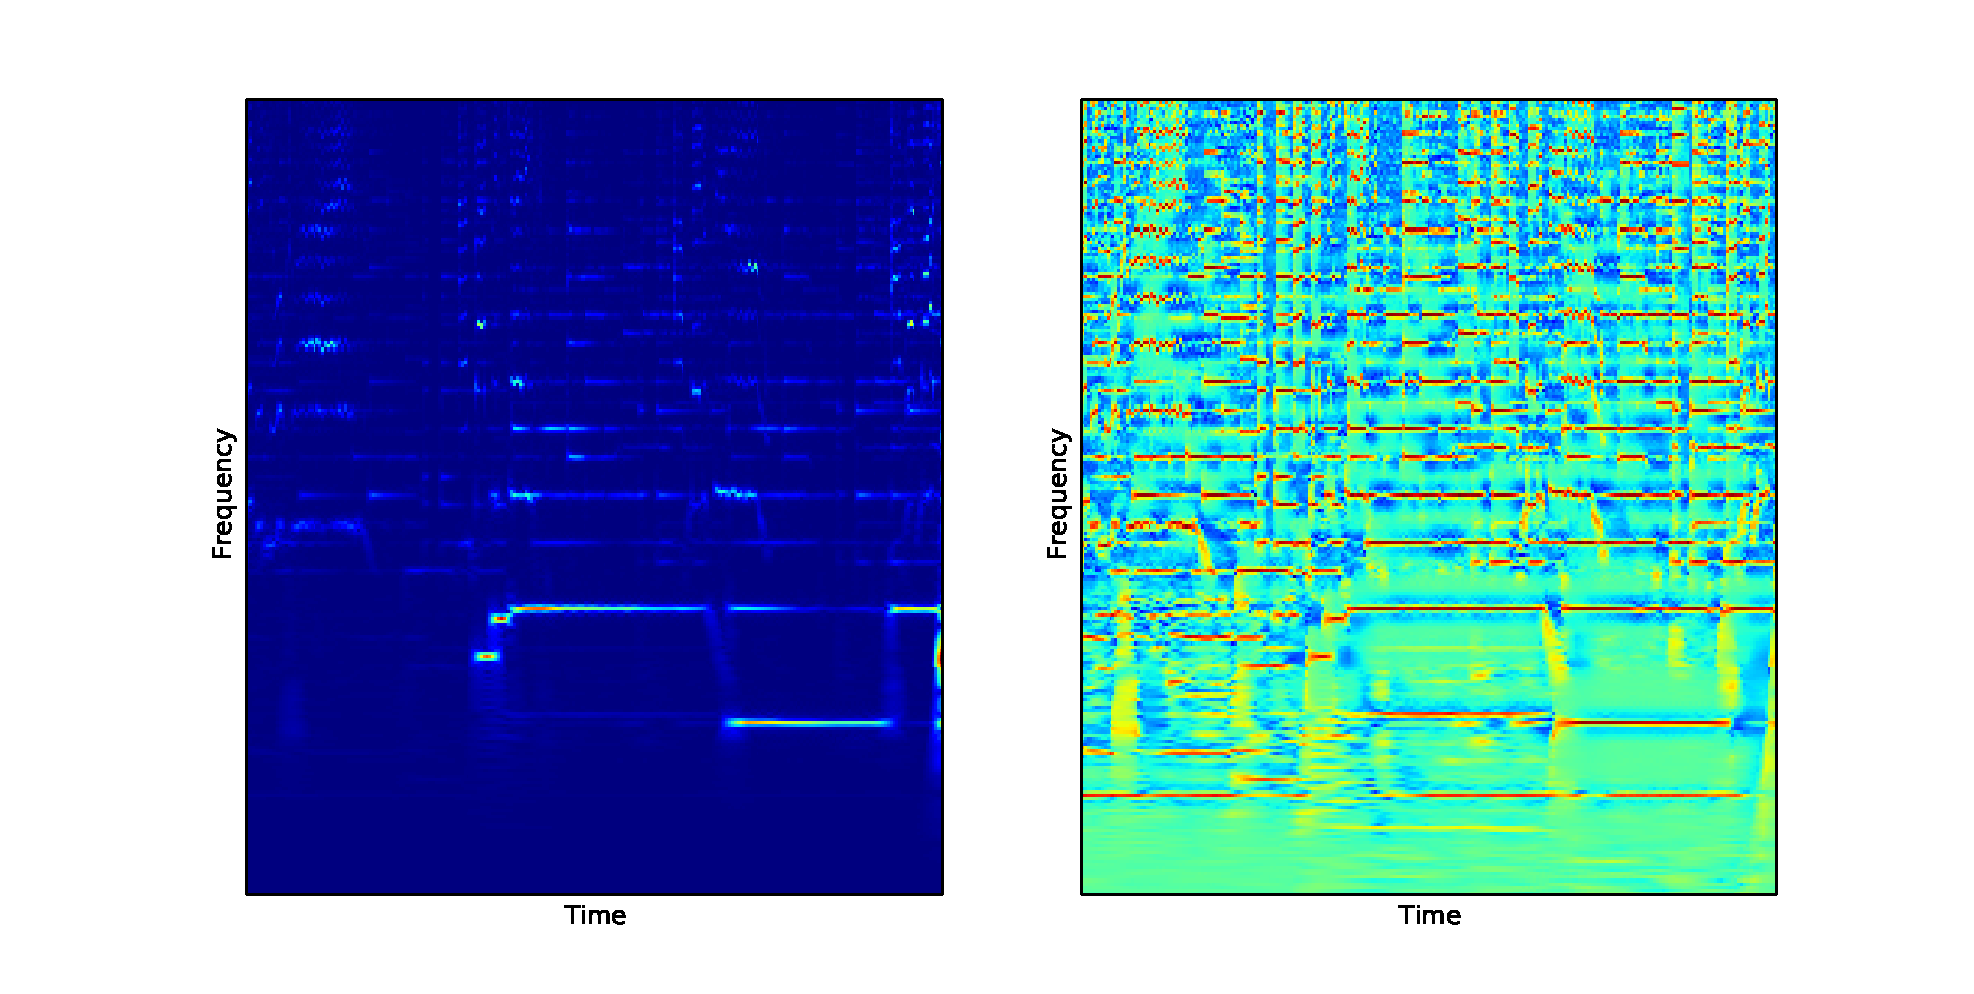
\includegraphics[width=5in]{cqt_compare}
\caption{The visible effects of octave-dependent LCN, before (left) and after (right).}
\label{fig:lcn_mods}
\end{figure}


\subsubsection{Designing a Root-Invariant Classifier}
\label{subsubsec:root_invariance}
One of the key findings from the previous study of deep networks for ACE, consistent with previous research, is the importance of enforcing or encouraging root-invariance in the model.
With GMMs, this is typically achieved by rotating all data, i.e. chroma features, to the same root and fitting a model for each quality.
Then, when applying the model, likelihoods are estimated for each root by circularly rotating chroma through all twelve positions to recover the full space of chord classes.
In our previous work on chord recognition, this concept was mimicked by rotating the data in the input domain.
While it led to improved results, rotating the data is less than ideal for at least two reasons.
One, it is an implicit, rather than explicit, association between classes, and the model is tasked with learning these redundant relationships.
In the case of chord recognition, the model needs to learn the same behavior 12 times over, to represent each quality in every root.
Two, rotating data in the input space may create unnatural artifacts in the kinds of data the model learns to expect, and it is not clear what, if any, side effects this may have.
It is assumed that this does not fundamentally change the latent distribution of the data used for training, but it may cause a mismatch with real data at test time.

An alternative to rotating the data, as convolutional networks have amply demonstrated, is to build the invariance directly into the architecture.
This is realized here by defining a fully convolutional model, such that the classifier's weights for each quality are shared over all roots; a diagram of this configuration is given in Figure \ref{fig:fullconvnet}.
Simplifying conceptually, this proceeds as follows: the penultimate representation is designed to yield a matrix with shape $(12 \times N)$, corresponding to the number of pitch classes and the chosen output dimensionality of the second to last layer, respectively; the chord classifier is then applied by taking the inner product with a weight matrix with shape $(N \times 13)$, corresponding to the dimensionality of the previous layer and the number of chord qualities, respectively.
For ease and efficiency this is implemented as a convolution, but the result is equivalent.
This produces a $(12 \times 13)$ matrix, which is flattened to represent the 13 qualities in all possible roots.
The no-chord condition is not captured by this operation, however, and a separate fully connected layer is applied in parallel to the flattened penultimate representation to estimate this class independently, which is then concatenated to the chord estimator.
Finally, this combined representation of 157 classes is normalized by the softmax operation, producing a probability mass function over all classes.

\begin{figure}[!t]
\centering
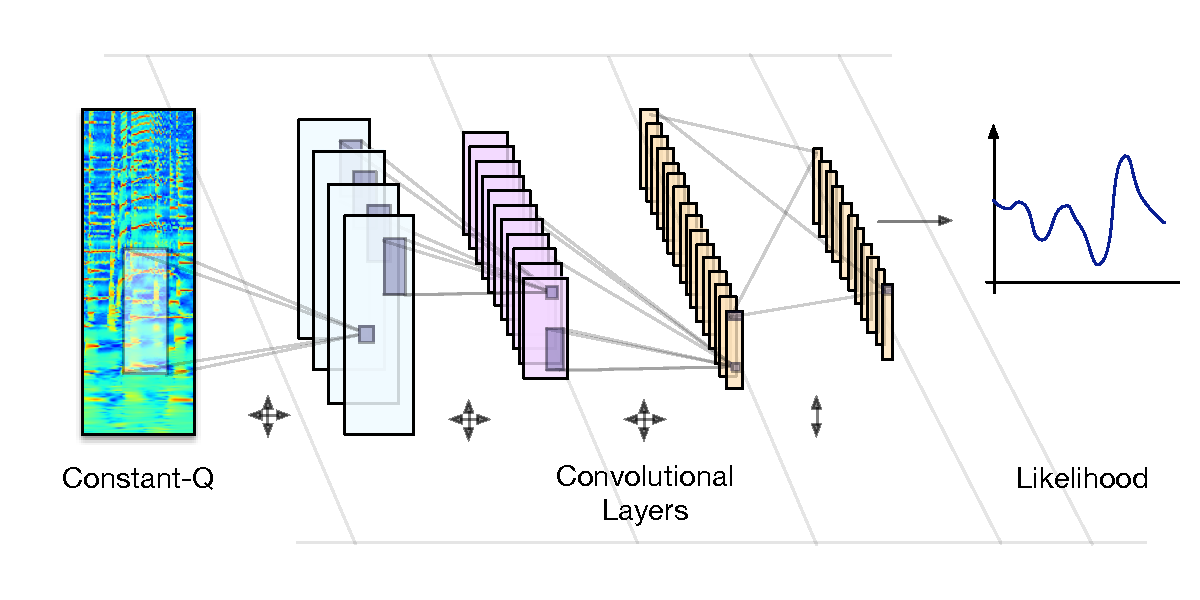
\includegraphics[width=5in]{fullconvnet}
\caption{A Fully Convolutional Chord Estimation Architecture.}
\label{fig:fullconvnet}
\end{figure}

% Additionally, we consider a variety of model complexities, defined in the following table:


\subsubsection{Correcting Bias with Scaled Likelihood Estimation}
\label{subsubsec:scaled_likelihood_estimation}
Having defined the output of the model as a probability function, it is trivial to again optimize the parameters to the negative log-likelihood over the dataset.
However, there are two difficulties that prohibit the uniform presentation of classes, as in previous work.
First, due to the increased number of classes, minibatches would either need to consist of many datapoints, increasing the processing time of each batch, or the learning rate would need to be smaller or diminishing over time to prevent oscillation, increasing the number of iterations necessary to converge.
To the latter point, it is easy to imagine scenarios where gradient descent wobbles back and forth between updates, as each batch pulls the parameters in a slightly different direction.
The other challenge this raises is a result of the considerable class imbalance, where uniform presentation would spend too much time on minority classes, while slowly the full extent of the majority classes.

The solution to this problem is found in Bayes' theorem, where the network is understood as yielding a class posterior probability, $P(Y|x)$, for the chord class, $Y$, given the observation, $x$:

\begin{equation}
P(x|Y) = \frac{P(Y|x)*P(x)}{P(Y)}
\end{equation}

The observation likelihood, $P(x|Y)$, is then a function of the posterior, the class prior, $P(Y)$, and probability of the observation itself, $P(x)$.
This final quantity is independent and thus can be ignored:

\begin{equation}
P(Y|X) \varpropto \frac{P(X|Y)}{P(Y)}
\end{equation}

While the deep network is trained to produce the class posterior, the class prior can be measured empirically over the training set, and divided out after the fact.
Referred to as \emph{scaled likelihood estimation}, this strategy has proven effective at reducing the effects of class imbalances in the functionally related domain of automatic speech recognition \cite{Deng, others}.
Notably, scaled likelihood estimation is particularly attractive here because it scales well with the number of estimated classes.

As a final comment, a possible pitfall when applying likelihood scaling is a matter of numerical stability arising from the least represented classes, or classes that might not even occur in the training set.
Whereas this can be mitigated with pseudo-counting \cite{?} --setting an heuristically determined, non-zero lower bound-- the class prior here is computed by counting each observation toward the same quality in all roots.
Though this prior could be seen as a coefficient vector to optimize in a more direct way, we find this approach works reasonably well in practice.


\subsubsection{Convolutional Dropout}
\label{subsubsec:conv_dropout}

Here, we extend the principles of dropout, discussed in Chapter \ref{chp:deep_learning}, to 3D convolutions.
In the weight-matrix case, training with dropout effectively ignores activations of an transformed output, setting them to zero.
Considering each output coefficient as a measure of activation for a given ``feature'', the act of dropout can be interpretted as sub-sampling the feature extractors learned by the model.

By extension, there are two ways the same principle could be applied in the case of 3D convolutions: over an entire 3D kernel, or distributed among all 2D receptive fields among all kernels.
We opt for the former as a trade-off in the degree of randomness dropout introduces to the training processes; the merits of one approach over another are left for future work.
Expressed formally, the $i^{th}$ kernel, $W_i$, can be masked with probability $p$, resulting in the possibly empty feature map, $Z_i$:

\begin{equation}
% \label{eq:conv_dropout}
Z_i = binomial(p) * h(X \circledast W_i + b_i) / (1.0 - p)
\end{equation}

\noindent where the output is also scaled by the complement of the probability.
Here, it is expected that each kernel learns a collection of feature extractors that, on average, work well together.
In the language of coadaptation, the tensor can be seen as a ``team'' of feature detectors, and as such correlations are broken up at this mid, as opposed to global, level.

There are two small implementation details worth noting.
First, the same parameters in the model are dropped out over the entire batch, and not separately for each datapoint in the batch.
In the bagging and model selection interpretation of dropout, this is analagous to updating one different model at each update step; the alternative effectively updates several models simultaneously.
Again, future work is necessary to determine the advantages of one approach versus another, but we prefer the single-select approach for its parallels to coordinate block descent \cite{somebody}.
Additionally, the original proposal of dropout suggests that the activations of all outputs be halved when using the full model at test time.
We find this somewhat cumbersome, and, as indicated in Eq. \ref{eq:conv_dropout}, scale \emph{up} the parameters during training, allowing models in test to be agnostic of dropout.


\subsubsection{Training and Early Stopping}
\label{subsubsec:early_stopping}

In contrast to the previous study, which converged to a stable result in a few thousand iterations, it takes considerably more effort to train models for this task, on the order of approximately 100k iterations.
Dropout, as predicted, takes roughly 4 to 5 times this amount to reach a maximal result.
Given the lengthy run time, we checkpoint parameters every 1k iterations during training and frame early stopping as a brute-force search over a finite set of parameter configurations.
Due to the application of Viterbi and the coupling with the self transition penalty, validation is non-trivial and computationally expensive.
Therefore, exhaustive validation is performed every 10k iterations, starting at 5k.
The best model and self-transition penalty are chosen by finding the configuration with the highest harmonic mean between the overall $f_1$ and average quality $f_1$ scores.


\subsubsection{Viterbi Post-filtering}
\label{subsubsec:viterbi}

Though somewhat standard at this point in ACE research, it is worthwhile to properly formalize the HMM-based post-filtering approach used here, given its considerable impact on system performance.



\subsection{Quantitative Results}
\label{subsec:quantitative_results}

Following from the setup defined above, we train a set of models for four dropout values, $p_{dropout} \in \{0.0, 0.125, 0.25, 0.5\}$, across five folds of the data.
Note that when $p_{dropout} = 0.0$, this is equivalent to training a model without dropout.
First, we are curious to investigate if and how the weight tying in the classifier has enforced the notion of root invariant representations.
% TODO: Observe that it learns a root invariant representation of qualities
% Distance matrix between qualities
% Ave vectors for same qualities in different roots

The
Concerning the question of performance, the recall averages across folds are given in the following table, using with the system and evaluation methodology presented in Cho \cite{Cho2014PhD}:

\begin{table}[h]
\begin{center}
\caption{Comparing chord symbol recall with a state of the art system.}
\label{tab:base_stats}
\begin{tabular}{l | c | c}

                      & Overall & Quality-wise  \\
\hline
Cho (2014)            & 62.41 & 47.31 \\
\hline
$p_{dropout} = 0.0$   & \textbf{67.37} & 41.02 \\
$p_{dropout} = 0.125$ & 65.53 & 48.15 \\
$p_{dropout} = 0.25$  & 64.91 & \textbf{53.39} \\
$p_{dropout} = 0.5$   & 63.92 & 52.13 \\
\hline
\end{tabular}
\end{center}
\end{table}

Based on this data, the different deep network models significantly out-perform the state of the art in large vocabulary ACE, some in slightly different ways.
The model trained with $p_{dropout} = 0.0$ does considerably better on the overall dataset by nearly $5\%$, but performs much worse on the quality-wise measure.
All dropout models recover this deficiency in the quality-wise recall surpassing state of the art, at the slight expense of overall recall.
Of the four, $p_{dropout} = 0.25$ is produces the best trade-off between the two metrics, yielding gains of $2\%$ and $6\%$ for the overall and quality-wise metrics, respectively.

If we were to stop here, it would give the impression that deep learning has once again trumped the previous benchmark.
However, there are other metrics to consider which tell a far more complex story of how these models perform.
The results of all metrics defined previously --precision, recall, and $f_1$ score, both overall and quality-wise-- are given in the following table:

\begin{table}[h]
\begin{center}
\caption{A more complete picture of system performance, contrasted against state of the art.}
\label{tab:base_stats}
\begin{tabular}{l | c c c | c c c |}
                      & \multicolumn{3}{c}{Overall} & \multicolumn{3}{c}{Quality-wise} \\
                      & Prec    & Rec.    & $f_1$   & Prec.     & Rec.      & $f_1$    \\
\hline
Cho (2014)            & 78.05   & 62.41   & 68.95   & 54.77     & 47.31     & 48.46    \\
\hline
$p_{dropout} = 0.0$   & 76.09   & 67.37   & 70.81   & 61.59     & 41.02     & 47.00    \\
$p_{dropout} = 0.125$ & 76.75   & 65.53   & 70.22   & 47.28     & 48.15     & 46.34    \\
$p_{dropout} = 0.25$  & 77.77   & 64.91   & 70.21   & 48.35     & 53.39     & 47.54    \\
$p_{dropout} = 0.5$   & 78.06   & 63.92   & 69.28   & 47.40     & 52.13     & 46.77    \\
\hline
\end{tabular}
\end{center}
\end{table}

Having more results from which to draw conclusions, a few interesting trends materialize.
Most noticeable is that despite the fluctuation in recall across models, the $f_1$ scores are all quite close; however, in this case, the previous system has the highest quality-wise score.
As a result, any rise or fall in recall is generally traded for a comparable shift in precision going the other direction.
This is most stark in the quality-wise measures for the model where $p_{dropout} = 0.0$.
It manages the lowest recall of any model, but also the highest precision by a large margin.
Interpreting the significance of this result, while this model may miss more instances of some chords, likely corresponding to the minority classes, it generally offers a higher degree of confidence in its estimations across qualities.
Additionally, while it at first seemed that dropout contributed significantly to improving the quality-wise measures, we see now that it primarily shifts the bias point from higher precision to higher recall, and the $f_1$ are within the same close margin.


TODO: Quality-wise recall bar plot, over four models
Run the other 4 folds for the 4 dropout conditions for the XXL model
Isn't TMC's system run on all 5 folds? where is this data


To continue developing a deeper understanding of these quality centric statistics, the top-5 confusions and corresponding recall percentages, rotated relative to C, are given in Tables \ref{tab:baseline_confs}-\ref{tab:dropout_p0x25_confs} for the baseline, no-dropout, and $25\%$-dropout models.
These results are tabulated by rotating the actual chord name to its equivalent quality in C, and applying the same rotation to the estimated label, thus preserving relative errors.
Interestingly enough, though the models are all roughly in the same performance range, they do so through very different means.


\begin{table}[h]
\begin{center}
\begin{scriptsize}
\caption{Top-5 relative confusions for Cho 2014}
\label{tab:baseline_confs}
\begin{tabular}{c || c | c | c | c | c |}
\hline
Actual & 1 & 2 & 3 & 4 & 5 \\
\hline
C:maj (69.45) &    C:7 ( 5.84) &   G:maj ( 3.02) &  C:maj7 ( 2.79) &   F:maj ( 2.71) &  C:sus4 ( 1.86) \\
  C:min (64.02) & C:min7 (11.98) &   C:maj ( 3.25) &  Eb:maj ( 3.12) &  C\#:min ( 2.62) &     C:7 ( 1.65) \\
 C:maj7 (65.38) &  C:maj (16.93) &  C:maj6 ( 1.94) &   G:maj ( 1.83) &  A:min7 ( 1.22) &  C:sus2 ( 1.08) \\
 C:min7 (45.40) &  C:min (24.75) &     C:7 ( 7.32) &  Eb:maj ( 3.23) &  Bb:maj ( 2.57) &     F:7 ( 1.49) \\
    C:7 (51.96) &  C:maj (19.81) &  C:sus4 ( 5.06) &   C:min ( 3.49) &       N ( 1.87) &   F:maj ( 1.84) \\
\hline
 C:maj6 (25.55) &  C:maj (14.60) &  A:min7 (12.49) &  C:sus2 ( 9.95) &  C:maj7 ( 7.76) &   A:min ( 7.57) \\
 C:min6 (34.96) & C:min7 (17.77) &     F:7 (13.76) & A:hdim7 ( 7.28) &   C:min ( 5.10) &   F:maj ( 3.20) \\
  C:dim (48.35) & C:hdim7 ( 7.03) &   C:min ( 5.73) &  C:min7 ( 5.25) &   F:maj ( 3.37) &  C:maj6 ( 3.24) \\
  C:aug (42.03) &  C:maj (18.63) &     C:7 ( 8.79) &   E:aug ( 6.21) &  C\#:min ( 5.94) &  C:maj7 ( 5.11) \\
 C:sus4 (46.64) &  C:maj (27.56) &   F:maj ( 5.61) &     C:7 ( 4.16) &  F:sus2 ( 4.01) &  Bb:maj ( 2.19) \\
 C:sus2 (72.32) &  C:maj (17.40) &  C:maj7 ( 6.13) &  D:sus4 ( 1.39) &   D:min ( 0.92) &  C:sus4 ( 0.81) \\
 C:dim7 ( 0.00) &  A:dim (35.59) &   A:min (18.13) &  A:maj7 (12.07) &   C:dim ( 8.77) &     A:7 ( 5.21) \\
C:hdim7 (36.32) &    C:7 (12.08) &  C:min7 ( 9.61) & Eb:min7 ( 6.63) &     F:7 ( 6.20) &  Eb:min ( 6.13) \\
\hline
      N (57.15) &  D:maj ( 2.54) &   E:maj ( 2.40) &   C:maj ( 2.29) &   G:maj ( 2.24) &   A:maj ( 2.21) \\
\hline
\end{tabular}
\end{scriptsize}
\end{center}
\end{table}


\begin{table}[h]
\begin{center}
\begin{scriptsize}
\caption{Top-5 relative confusions for $p_{dropout} = 0.0$}
\label{tab:baseline_confs}
\begin{tabular}{c || c | c | c | c | c |}
\hline
Actual & 1 & 2 & 3 & 4 & 5 \\
\hline
C:maj (79.86) &     C:7 ( 3.41) &        N ( 2.84) &    F:maj ( 2.39) &    G:maj ( 1.85) &   C:maj7 ( 1.29) \\
C:min (63.90) &  C:min7 (11.54) &    C:maj ( 7.14) &   Eb:maj ( 3.82) &        N ( 2.39) &    F:maj ( 1.85) \\
C:maj7 (60.79) &   C:maj (25.60) &    G:maj ( 3.26) &   A:min7 ( 1.46) &    E:min ( 1.18) &   C:maj6 ( 1.04) \\
C:min7 (46.25) &   C:min (24.29) &    C:maj ( 9.71) &   Eb:maj ( 4.46) &   Bb:maj ( 2.21) &    F:maj ( 1.93) \\
C:7 (35.48) &   C:maj (46.47) &        N ( 3.38) &    F:maj ( 2.54) &   Bb:maj ( 1.35) &   C:sus4 ( 1.18) \\
\hline
C:maj6 (20.90) &   C:maj (49.92) &   C:maj7 ( 7.43) &   C\#:maj ( 3.77) &        N ( 3.04) &   F:maj7 ( 1.82) \\
C:min6 (13.30) &   C:min (29.45) &   C:min7 (26.06) &      F:7 ( 9.32) &    C:maj ( 7.66) &      B:7 ( 6.65) \\
C:dim (36.12) &   C:min (15.53) &     Ab:7 ( 7.87) &        N ( 6.32) &   C:dim7 ( 4.20) &    C:maj ( 3.63) \\
C:aug (22.24) &   C:maj (34.69) &      C:7 ( 8.03) &   C\#:min ( 7.58) &   C:maj7 ( 6.11) &    F:min ( 2.77) \\
C:sus4 (25.95) &   C:maj (50.13) &      C:7 ( 7.04) &    F:maj ( 3.90) &        N ( 2.90) &   Bb:maj ( 1.74) \\
C:sus2 (61.81) &   C:maj (28.10) &   C:maj7 ( 4.36) &        N ( 1.40) &    G:maj ( 1.23) &   C:sus4 ( 0.98) \\
C:dim7 ( 0.00) &   A:maj (44.64) &    A:dim (22.38) &    A:min (20.93) &        N ( 4.33) &    B:maj ( 3.00) \\
C:hdim7 (32.09) &  Eb:min (10.47) &   C:min7 ( 9.13) &    C:maj ( 6.21) &     Ab:7 ( 6.02) &      F:7 ( 5.96) \\
\hline
N (75.48) &   C:maj ( 2.85) &    D:maj ( 2.06) &    A:maj ( 1.90) &    F:maj ( 1.67) &   Bb:maj ( 1.6105) \\
\hline
\end{tabular}
\end{scriptsize}
\end{center}
\end{table}


\begin{table}[h]
\begin{center}
\begin{scriptsize}
\caption{Top-5 relative confusions for $p_{dropout} = 0.25$}
\label{tab:baseline_confs}
\begin{tabular}{c || c | c | c | c | c |}
\hline
Actual & 1 & 2 & 3 & 4 & 5 \\
\hline
C:maj (70.08) &     C:7 ( 5.91) &       N ( 3.43) &  C:maj6 ( 3.01) &  C:maj7 ( 2.56) &   F:maj ( 1.89) \\
  C:min (58.18) &  C:min7 (18.31) &   C:maj ( 3.80) &       N ( 3.12) &  C:min6 ( 2.26) &     C:7 ( 2.03) \\
 C:maj7 (72.59) &   C:maj (12.14) &  C:maj6 ( 2.71) &  G:maj6 ( 2.45) &  A:min7 ( 1.44) &       N ( 1.02) \\
 C:min7 (56.51) &   C:min (18.48) &     C:7 ( 6.24) &       N ( 2.36) &   C:maj ( 1.66) &  Eb:maj ( 1.20) \\
C:7 (50.51) &   C:maj (26.03) &       N ( 4.87) &  C:sus4 ( 2.37) &  C:maj6 ( 1.88) &  G:min7 ( 1.75) \\
\hline
 C:maj6 (41.29) &   C:maj (19.34) &  C:maj7 (10.00) &  C\#:maj ( 6.52) &  C:sus2 ( 5.03) &  A:min7 ( 3.27) \\
 C:min6 (55.99) &  C:min7 (24.22) &   C:min ( 7.48) &     B:7 ( 5.34) &     F:7 ( 0.95) &  D:min7 ( 0.83) \\
  C:dim (38.31) &  C:dim7 (12.84) & C:hdim7 (10.05) &  C:min6 ( 6.49) &   C:min ( 4.74) &       N ( 4.30) \\
  C:aug (46.23) &   C:maj (13.97) &     C:7 ( 8.09) &       N ( 4.86) &  C\#:min ( 4.81) &  Ab:aug ( 4.52) \\
 C:sus4 (38.43) &   C:maj (31.54) &     C:7 (12.63) &  C:sus2 ( 1.72) &  F:sus2 ( 1.66) &   F:maj ( 1.53) \\
 C:sus2 (77.59) &   C:maj (16.37) &  C:maj7 ( 3.17) &     C:7 ( 0.91) &   G:maj ( 0.77) &  D:sus4 ( 0.38) \\
 C:dim7 ( 0.00) &   A:dim (39.22) &   A:maj (31.40) &   A:min (11.91) &       N ( 5.17) &   C:dim ( 4.93) \\
C:hdim7 (65.10) &  C:min7 ( 8.95) &   C:min ( 3.95) &    Ab:7 ( 3.47) & C\#:min7 ( 3.41) &     C:7 ( 2.92) \\
\hline
      N (76.56) &   C:maj ( 2.14) &   E:maj ( 1.42) &   A:maj ( 1.42) &   D:maj ( 1.35) &   G:maj ( 1.23) \\
\hline
\end{tabular}
\end{scriptsize}
\end{center}
\end{table}

What we see from this confusion analysis is that the errors made by these systems are often musically plausible, and in some cases it might be difficult to call them errors.
A \texttt{C:dim7}, for example, itself contains a \texttt{C:dim} triad.
From both a system design and evaluation standpoint, this motivates some kind of hierarchical representation, where triads are predicted at a coarser level than tetrads, e.g. $\{\texttt{C:dim}, \texttt{C:dim7}, \texttt{C:hdim7}\} \implies \texttt{C:dim}$.


\subsection{Qualitative Analysis}
\label{subsec:qualitative_analysis}

In the previous subsection we were able to address many of the research questions posed.
The final question ---is system behavior consistent with quantitative evaluation?--- can only be investigated through qualitative analysis.
Returning to the metrics presented in Section \ref{subsec:evaluation_methodology}, there are two dimensions of interest on which they can be examined: the averaging of measures over qualities, and the comparison function between chord names.

% Is quality-wise even a good measure?
It was observed during training that achieving a good balance between overall and quality-wise performance is especially challenging.
Observing these statistics over the various checkpoints in parameter selection for validation reveals a curious trend: very small changes in a quality-wise metric can result in an enormous differential in the overall one.
This makes perfect sense in hindsight, and is illustrated in Figure \ref{fig:bigswing}.
Due to the large imbalance of classes, a tiny shift in a decision boundary between two closely related classes, such as \texttt{C:maj} and \texttt{C:maj6}, will affect the different measures disproportionately.
This calls into question somewhat the stability of quality-wise measures, and the relative weight they should receive when comparing systems on this kind of metric.
Is it undesirable for a system to miss rare chords in favor of those that occur most frequently if it results in better overall performance?
There may be no definitive answer to such a question, instead being determined as a function of a system's design and target use case.
It is a valuable goal to make sure that computational systems perform well across all kinds of data and not just the most common cases.
However, it seems equally important to avoid measures that introduce other, perhaps artificial, biases in model selection.
% This is known as a macro-average (right), and it must be a known issue. How do others get around it? Perhaps a non-linear combination would stabilize this (geo-mean, log-weighting of contributions, etc).

\begin{figure}[!t]
\centering
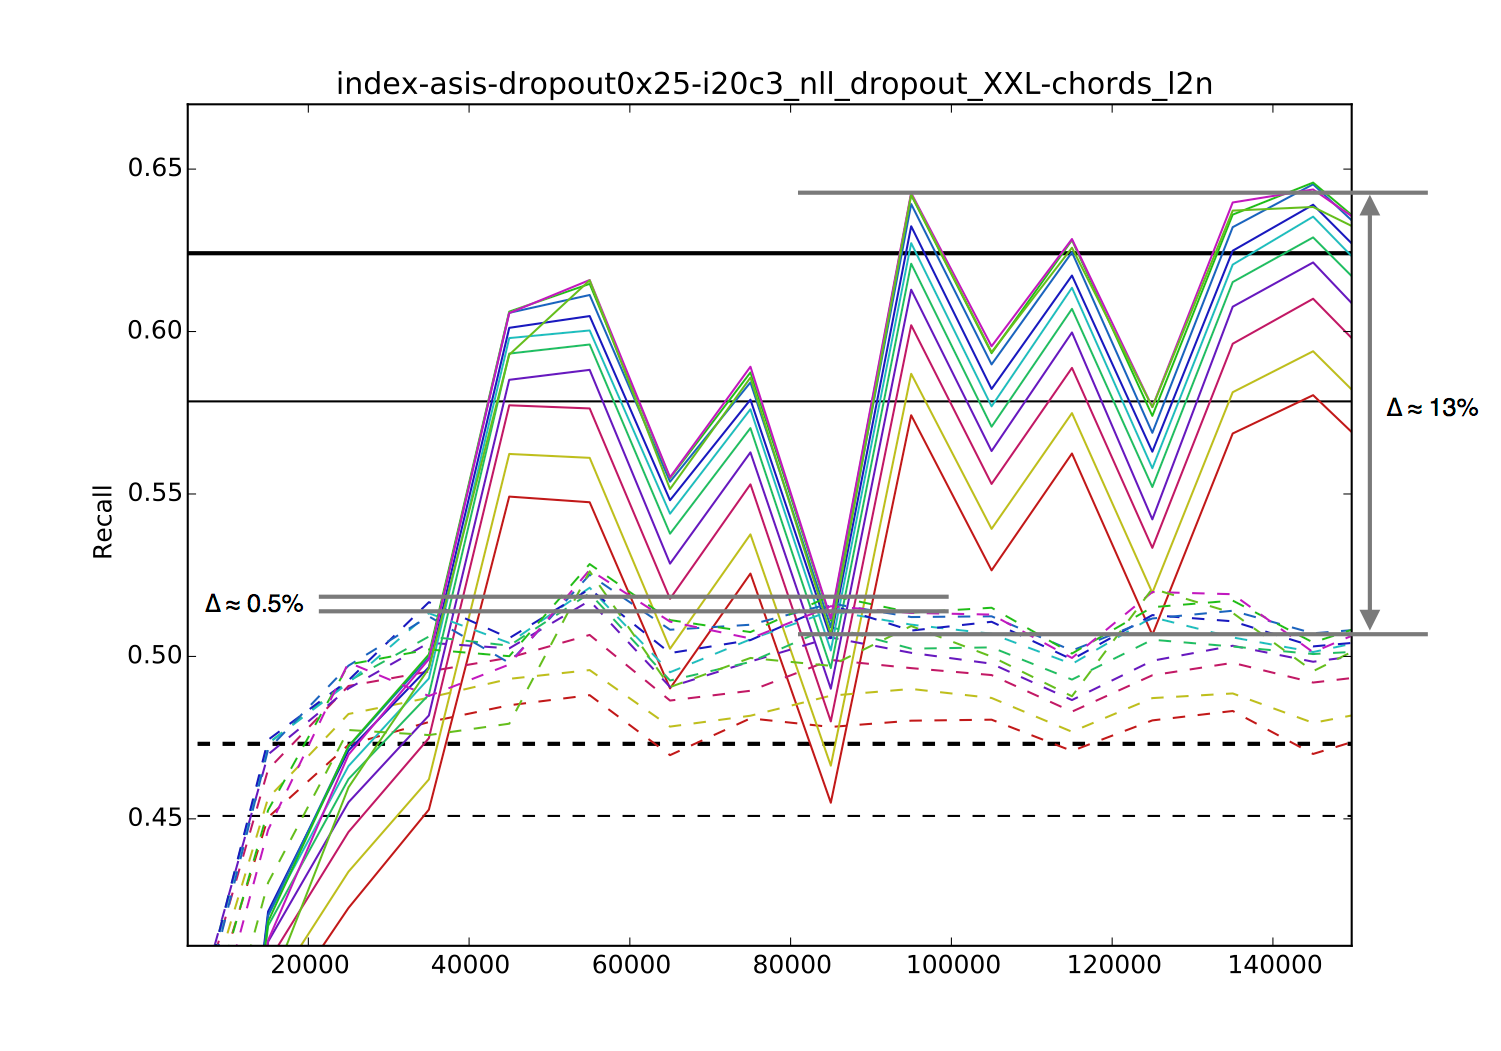
\includegraphics[width=5in]{bigswing}
\caption{Validation performance as a function of iteration; overall (solid) and quality-wise (dashed) recall are shown for multiple self-transition penalties.}
\label{fig:bigswing}
\end{figure}

% Considering the comparison function
The choice of comparison function is a slightly more complex dimension to investigate.
As shown in the previous section, the confusions made by these systems are predominantly between similar, and in some cases harmonically valid, chord names.
Notably, the idea has been proposed in the past that softer evaluations measure could be used to better characterize harmonic similarity, such as pitch recall or comparing only the first two or three intervals in a chord \cite{Harte2010PhD}.
Neither of these approaches have seen much traction in the community, nor are they satisfying from a research standpoint.
Both approaches suffer from the deficiency that they may artificially inflate performance statistics without necessarily leading to fundamentally better systems.
In both cases, a system that fails to produce any strictly ``correct'' answer could receive the same score as a system that reproduces the ground truth exactly.
Additionally, grounding softer comparisons in music theory can require extra information about the specific key and harmonic function of the chord, information that grouth truth transcriptions may not contain explicitly.
For example, \texttt{C:maj} and \texttt{C:maj7} are both syntactically valid and functionally equivalent in the key of $C_{major}$, as these chords build on the tonic.
In $F_{major}$, conversely, a \texttt{C:maj7} is harmonically invalid; here, C is the fifth scale degree, or dominant, and therefore \texttt{C:maj} and \texttt{C:7} would be functionally equivalent (hence the term ``dominant'' 7th chord).
The resulting conundrum in ACE evaluation is that while strict chord comparisons are not necessarily well aligned with subjective experience, alternative strategies toward softer comparisons leave something to be desired.
Therefore, how might we better encode if and when different chord names are acceptable?

% Pull in multiple perspectives : Introducing the Rock Corpus
One way to address this is to call into question the validity of the ground truth transcriptions themselves.
Recall that the various chord annotation collections used in development and evaluation here were all curated through a review process, whereby disagreements or judgement calls where ironed out as ``errors'', in the effort of producing singular chord names over time.
As a result, the notion of ground truth is baked into the data itself.
Fortunately, the \emph{Rock Corpus} dataset, first introduced in \cite{deClerqc2010}, is a set of, at the time of writing, 200 popular rock tracks with time-aligned chord and melody transcriptions performed by two expert musicians.
Ironically, this collection of chord transcriptions has seen little use in the ACE literature, as its initial release lacked timing data for the transcriptions, and the chord names are provided in a Roman Numeral syntax.
A subsequent release fixed the former issue, however, in addition to doubling the size of the collection from 100 to the now 200 tracks.
The latter issue is more a matter of convenience, as key information is provided with the transcriptions and this format can be translated to absolute chord names, consistent with the syntax in Section \ref{subsec:chord_syntax}.
This dataset provides a previously uncapitalized opportunity to explore the behavior of ACE systems as a function of multiple reference transcriptions.

% What happens if the ground truth changes?
We first consider the effects of choosing a different ground truth.
Using the same fuzzy string matching described above, we identify 45 tracks in the collection that are also in the Rock Corpus, and we can look at what happens if either of these new annotations were used as ground truth.
You get big swings in accuracy depending on which perspective you end up with, and in some sense, they're both equally valid.
Concurrent opinions are different from sequential opinions; this is known as ``anchoring'' and causes hysteresis in annotation.
For example, ``Human A says X, human B doesn't disagree'' doesn't entail ``Human B says Y, human A disagrees''.

% What if either is ground truth? We can look at C(A, B) vs max(C(A, M), C(B, M)), over the rock corpus alone, to obtain many datapoints.
%
% Three elements fall out:
%








\subsection{Conclusions}
\label{subsec:conclusions}

% Quantitative observations
Overall, considering the research questions posed, we find that the deep learning approach outperforms the state of the art in the typical measures of quantitative evaluation.
We

% Qualitative observations
We need to develop better means of curating datasets such that objective measures better correspond with subjective experience.


\section{Summary}
\label{sec:summary}

In this chapter we have thoroughly explored the application of deep learning methods to the classic MIR task of ACE.
By standard evaluation practices, we demonstrate competitive performance in a Major-minor formulation of the task, and an improvement over the state of the art with considerably larger chord vocabularies.
